\chapter{Variationelle Modelle für Phasenübergänge}{\label{ch:calcvarphase}}
Im Folgenden setzen wir fest:
\begin{itemize}
    \item \(\Omega\) als ein beschränktes Lipschitz-Gebiet im \(\mathbb{R}^n\).
\end{itemize}
\section{Flüssig-flüssig Phasenübergänge}{\label{sec:flflphase}}
\subsection{Das Becker Modell}{\label{subsec:becker}}
Wir werden uns nun einer mathematischen Beschreibung von Phasenübergängen widmen. Zunächst sind wir bei einer derartigen Phasentrennung natürlich interessiert an der zugrundeliegenden Energie im Phasenübergang. R. Becker untersuchte dieses Problem in \cite{BeckerKeimbildung}, als er die Keimbildung in metallischen Mischkristallen genauer betrachtete. Unter Berücksichtung etwaiger physikalischer (Erhaltungs-)Gesetze ergab sich daraus folgendes mathematisches Modell (mathematisch präzesierte Version von \cite{ambrosio2000variational}[Seite 5]) für die anisotropische Energie auf der "Sprungmenge" \(S\):\\[0.5cm]
\pgfsetfillopacity{0.1}\colorbox{generalYellow}{\begin{minipage}{16cm}{\textcolor{black}{\pgfsetfillopacity{1}}{\label{def4.1}}}
\textbf{Definition 4.1 (Becker Modell, 1938):} Betrachte zwei nicht homogene Flüssigkeiten in \(\Omega\), die sich durch Oberflächenspannung voneinander seperieren. Wir betrachten hierzu den zulässigen Konfigurationsraum:
\begin{equation}
    \mathcal{A} := \{u : \Omega \to \{0,1\} \, | \, \int_{\Omega} u \, d\lambda^n = \lambda^n(V)\},
\end{equation}
wobei \(V \subset \mathcal{M}^n(\Omega)\) dem Raum der zweiten Flüssigkeit entspricht.
Die Phasentrennung bezeichnen wir mit \(S(u) \subset \mathcal{B}(\mathbb{R}^{n-1})\), auf welcher folgende Energie verteilt liegt:
\begin{equation}
    \mathcal{E}(u) := \sigma \mathcal{H}^{n-1}(S(u)),
\end{equation}
wobei \(\sigma\) die anisotropische Energie auf der Phasentrennung \(S(u)\) bezeichnet.
\end{minipage}}

\textbf{Bemerkung:} \begin{itemize}
\item Das Modell wurde ursprünglich für n=3 entwickelt, kann aber für beliebige endliche Dimension verallgemeinert werden.
\item \(\mathcal{H}^{n-1}(S(u))\) existiert, da in metrischen Räumen \((\mathcal{X},d_{\mathcal{X}})\) n-1-dimensionale Borelmengen auch \(\mathcal{H}^{n-1}\)-messbar sind. Der Grund hierfür ist, dass das Hausdorff-Maß als äußeres Maß das Caratheodory-Messbarkeitskriterium bezüglich \\ abgeschlossenen Teilmengen von \(\mathcal{X}\) erfüllt und sich alle Borelmengen als Kombination abgeschlossener Mengen unter \(\mathcal{B}\)-stabilen Mengenoperationen darstellen lassen.
\item \(S(u)\) lässt sich als Menge der Singularitäten (bzw. "Sprungmenge") von \(u\) auffassen, i.e. mathematisch exakt ist diese Menge definiert als (vergleiche hierzu [\ref{def2.24}, Definition 2.24]):
\begin{equation}
    S(u) := \bigcup_{i=1}^n \{x \in \Omega \, | \, u^-_i(x) < u^+_i(x)\}.
\end{equation}
\end{itemize}

\begin{figure}[label={fig:chmod}, caption={Phasentrennung von Sonnenblumenöl (gelb) und Wasser: Links eine Fotoaufnahme, rechts ein modellierter Querschnitt}] 
\begin{subfigure}{.4\textwidth}
  \centering
  \includegraphics[scale=0.2]{figures/PhaseTr-RL.pdf}
%%%%%%%%%%%%%%%%%%%%%%%%%
\end{subfigure}%
\(\, \,\)
  \begin{subfigure}{.4\textwidth}
  \centering
\begin{tikzpicture}
    \draw [name path = A] (-2,0) -- (-2,3);
    \draw [name path = B] (2,0) -- (2,3);
    \draw [name path = C] (-2,0) -- (0,0);
    \draw [name path = L] (0,0) -- (2,0);
    \draw [name path = D, ultra thick, red, bend left=20] (-2,3) to (0,3);
    \draw [name path = E, ultra thick, red, bend right=20] (0,3) to (2,3);
    \draw [name path = F] (-2,3) -- (-2,4);
    \draw [name path = G] (2,3) -- (2,4);
    \draw [name path = H, yellow, bend left=20] (-2,4) to (0,4);
    \draw [name path = I, yellow, bend right=20] (0,4) to (2,4);
    \draw [name path = J] (-2,4) -- (-2,5);
    \draw [name path = K] (2,4) -- (2,5);
    \tikzfillbetween [of=C and D]{blue, opacity=0.8};
    \tikzfillbetween [of=L and E]{blue, opacity=0.8};
    \tikzfillbetween [of=D and H]{yellow, opacity=0.8};
    \tikzfillbetween [of=E and I]{yellow, opacity=0.8};
    \draw [blue!80] (0,0) -- (0,3);
    \draw (-2.5,0.25) node {$\Omega$};
    \draw (3,1.5) [text=blue] node {0};
    \draw (3,3.5) [text=yellow] node {1};
    \draw (2.5,3) [text=red] node {S(u)};
    \draw [ultra thick] (-2,0) -- (-2,5);
    \draw [ultra thick] (-2,0) -- (2,0);
    \draw [ultra thick] (2,0) -- (2,5);
\end{tikzpicture}
%\caption{Phasentrennung für den Spezialfall von n=2: Zwei Flüssigkeiten in einem Becher \(\Omega\): Sonnenblumenöl (hier V, gelb) und Wasser (blau)}
\end{subfigure}%
\(\, \,\)
\begin{subfigure}{.4\textwidth}
  \centering
%\caption{Cauchy-Stresstensor für den Spezialfall von n=3: Zur Verdeutlichung des Stresstensors fehlt hier im Bild das Sonnenblumenöl. Hierbei stellen die \(\sigma_{ii}\) den Druck, sowie alle anderen Komponenten die sogenannte Schubspannung auf die (n-1)-dimensionale Untermannigfaltigkeit (hier Su) dar.}
%%%%%%%%%%%%%%%%%%%%%%%%%
\end{subfigure}
\end{figure}

\subsection{Das Cahn-Hilliard Modell}{\label{subsec:cahnhilliard}}
Nach Betrachtung des Becker-Modells könnte man auf die Idee kommen, dass wir den Phasenübergang von zwei nicht homogenen Flüssigkeiten zufriedenstellend analysiert haben. Doch das Becker-Modell erzeugt sowohl mathematische, als auch physikalische Probleme:
\begin{itemize}
    \item Im physikalischen Sinne setzt es voraus, dass die Oberflächenspannung von \(S(u)\) ausreicht, damit dieses invariant bezüglich Druck oder Temperatur bleibt. Natürlich ist das idealisiert und entspricht überhaupt nicht der wahren thermodynamischen Natur (Thermodynamik nach dem Stand Mai 2023).
    \item Mathematisch sind wir natürlich daran interessiert, dass im Allgemeinen die Gesamtenergie auf \(\Omega\) auf \(S(u)\) minimiert wird, i.e. \(S(u)\) besitzt eine so minimale Fläche wie möglich. Dem Konfigurationsraum des Becker-Modells zufolge setzten wir fest:
    \begin{equation}
        \int_{\Omega} u \,d\lambda^n = \lambda^n(V) =: m.
    \end{equation}
    Damit wir die Gesamtenergie minimieren können, müssen wir die Phasenseperation minimieren, i.e. wir suchen den Minimierer von:
    \begin{equation}
        \tilde{\mathcal{E}}(u) := \int_{\Omega} W(u) \,d\lambda^n,
    \end{equation}
    wobei \(W\) der doppelte Potentialtopf (stetige, positive Funktion) mit einzigen Nullstellen \(\alpha, \, \beta \in \mathbb{R}\), für die wir o.B.d.A. annehmen, dass \(0 < \alpha < \beta\) gilt. Zusammengefasst sind wir an \(\alpha \lambda^n(\Omega) \leq m \leq \beta \lambda^n(\Omega)\) mit einer Minimierung der Fläche zwischen \(\{u = \alpha\}\) und \(\{u = \beta\}\) interessiert. Wir sehen an dieser Problemstellung, dass wir auch keine mathematische zufriedenstellende Antwort mit der "Becker-Energie" \(\mathcal{E}(u)\) als Gesamtenergie erhalten werden. Genau gesprochen ist hier das Problem, dass wir für das Minimierungsproblem \(W\) um eine affine Translation modifizieren können, ohne das Minimierungsproblem zu beeinflussen. Wir erhalten unendlich viele Lösungen, ohne dabei allgemein das "minimale Flächenproblem" von \(S(u)\) in vernünftiger Weise berücksichtigen können (Wir werden in \ref{subsec:modicamortola} diesen Aspekt noch einmal aufgreifen und zeigen, wie man diesen korrekt löst.).
\end{itemize} 
J. Cahn und J. Hilliard verbesserten das Becker-Modell deshalb 1957 in \cite{CahnHilliard} wie folgt (mathematisch präzesierte Version von \cite{ambrosio2000variational}[Seite 5--6]):\\[0.5cm]
\pgfsetfillopacity{0.1}\colorbox{generalYellow}{\begin{minipage}{16cm}{\textcolor{black}{\pgfsetfillopacity{1}}{\label{def4.2}}}
\textbf{Definition 4.2 (Cahn-Hilliard Modell, 1957):} Betrachte zwei nicht homogene Flüssigkeiten in \(\Omega\), die sich \textit{bis auf \(\mathcal{H}^{n-1}\)-Nullmengen} durch Oberflächenspannung voneinander seperieren. Wir betrachten hierzu den zulässigen Konfigurationsraum:
\begin{equation}
    \mathcal{A} := \{u : \Omega \to [0,1] \, | \, \int_{\Omega} u \, d\lambda^n = \lambda^n(V) \},
\end{equation}
wobei \(V \subset \mathcal{M}^n(\Omega)\) wieder dem Raum der zweiten Flüssigkeit entspricht.
Die Phasentrennung \textit{als kontinuierlicher Vorgang} bezeichnen wir mit \(S(u) \subset \mathcal{B}(\mathbb{R}^{n-1})\), \textit{i.e. \(S(u)\) ist die Menge, auf der \(u\) \textbf{wesentlich} unstetig ist} (in Analogie zur Bemerkung unter dem Becker Modell überträgt sich die dortige Definition (bis auf einen Vorfaktor), indem man die approximative Stetigkeit dort bis auf eine \(\lambda^n\)-Nullmenge fordert). Als Gesamtenergie auf \(\Omega\) setzen wir dann fest:
\begin{equation}
    \mathcal{E}_{\epsilon}(u) := \epsilon^2 \int_{\Omega} |\nabla u |^2 \, d\lambda^n + \int_{\Omega} W(u) \, d\lambda^n \, \, \forall \epsilon > 0 \, \forall W \in \mathcal{C}(\mathbb{R}_0^+).
\end{equation}
Hierbei ist
\begin{equation}
\{W(u(x)) = 0\} = \{0,1\} 
\end{equation}
und man nennt \(W\) physikalisch auch einen doppelten Potentialtopf (Englisch: "Double well potential"; siehe Exkurs in \ref{sec:exwell}). Für kleine \(\epsilon\) entspricht der erste Summand der Energie der örtlichen Inhomogenität und der zweite Summand einer Phasenseperation, welche große Wahrscheinlichkeitsmasse in 0 und 1 annimmt.
\end{minipage}}

%%%%%%%%%%%%%%%%%%%%%%%%%%%%%%%%%%%%%%%%%%%%%%%%%%%%%%%%%%%%%%%%%%%%%%%%%%%%%%%%%%%%%%%%%%%%%%%%%%%%%%%%%%%%%%%%%%%%%%%%%%%%%%%%%%%%%%%%%%%%
\subsection{Zusammenhang von Becker und Cahn-Hilliard Modell: Modica-Mortola Theorem}{\label{subsec:modicamortola}}
Wenn wir als Gesamtenergie für das System die "Cahn-Hilliard-Energie" \(\mathcal{E}_{\epsilon}(u)\) festsetzen, sollte diese im Gleichgewichtszustand mit der "Becker-Energie" \(\mathcal{E}(u)\) übereinstimmen. Genau diesen Aspekt gilt es nun also zu verifizieren, wobei wir für dieses Problem der Theorie der \(\Gamma\)-Konvergenz bedienen werden. L. Modica und S. Mortola untersuchten 1977 Gradiententheorien für Phasenübergängen in \cite{mortola1977esempio} und stellten dabei in einem verallgemeinerten Rahmen fest, dass unter vernünftigen Voraussetzungen das Cahn-Hilliard Modell gegen das Becker Modell \(\Gamma\)-konvergiert. Grundsätzlich ist \(\Gamma\)-Konvergenz der Definition nach bereits invariant unter stetigen Perturbationen. Wir werden nun jedoch das Cahn-Hilliard Modell noch ein wenig weiter verallgemeinern, um ähnliche variationelle Probleme mit abzudecken. Genau genommen modifizieren wir:
\begin{equation}{\label{eq4.11}}
    u : \Omega \to [\alpha,\beta], \, \{W(u(x)) = 0\} = \{\alpha,\beta\},
\end{equation}
wobei \(0 < \alpha < \beta\). Ziel dieses Kapitels ist es nun, das Modica-Mortola Theorem zu beweisen, welches Folgendes besagt:\\[0.5cm]
\pgfsetfillopacity{0.1}\colorbox{generalYellow}{\begin{minipage}{16cm}{\textcolor{black}{\pgfsetfillopacity{1}}{\label{theo4.3}}}
\textbf{Satz 4.3 (Modica-Mortola, 1977):} Sei \(m \in \mathbb{R}\) beliebig, aber fest mit
\begin{equation}
    \alpha \lambda^n(\Omega) \leq m \leq \beta \lambda^n(\Omega).
\end{equation}
Betrachte folgendes Energiefunktional:
\begin{equation}
    \Fep(u) :=
    \begin{cases}
        \int_{\Omega} \epsilon |\nabla u|^2 + W(u(x)) \, d\lambda^n(x), \text{ falls }u \in W^{1,2}(\Omega) \\ +\infty, \text{ sonst}
    \end{cases},
\end{equation}
sowie die Oberflächenspannung
\begin{equation}
    \sigma := \int_{[\alpha,\beta]} \sqrt{W(u(x))}\, d\lambda^n(x),
\end{equation}
wobei \(W\) stetig und wie in \eqref{eq4.11}.\\
Weiter sei \(u_{\epsilon}\) die Lösung des variationellen Problems
\begin{equation}
    \Fep(u_{\epsilon}) = \min \{\Fep(u) \, | \, u \in L^1(\Omega), \, u \geq 0, \int_{\Omega} u(x) \, d\lambda^n(x)= m\}.
\end{equation}
\end{minipage}}
\newpage
\pgfsetfillopacity{0.1}\colorbox{generalYellow}{\begin{minipage}{16cm}{\textcolor{black}{\pgfsetfillopacity{1}}{\label{theo4.3b}}}
Falls für eine Familie reell positiver Zahlen \(\epsilon_h\) gilt, dass
\begin{equation}
    (\epsilon_h \to 0 \, \land \, u_{\epsilon_h} \to u_0 \in L^1(\Omega)),
\end{equation}
dann gilt:
\begin{enumerate}
    \item \(u_0(x) \in \{\alpha,\beta\}\) f. \(\lambda^n-\)f.a. \(x \in \Omega\),
    \item Der minimale Perimeter von \(\Omega\) wird für \(\alpha\) erreicht, i.e. es gilt:
    \begin{equation}
        E := \{x \in \Omega \, | \, u_0(x)=\alpha\}
    \end{equation}
    ist Lösung von
    \begin{equation}
        |D\chi_E |(\Omega) = \min \{|D\chi_B |(\Omega) \, | \, B \subseteq \mathcal{M}^n(\Omega), \, \lambda^n(B) = \frac{\beta \lambda^n(\Omega) - m}{\beta - \alpha}\},
    \end{equation}
    \item \(\frac{\mathcal{F}_{\epsilon_h}(u_{\epsilon_h})}{\sqrt{\epsilon_h}} \to 2\sigma |D\chi_E |(\Omega)\).
\end{enumerate}
\end{minipage}}

Für den Beweis benötigen wir einige Vorarbeit. Hierbei orientieren wir uns an dem originalen Beweis von L. Modica und S. Mortola, der in englischer Form in \cite{modica1987gradient} zu finden ist. Die Idee wird es sein, eine Art \(\Gamma\)-Konvergenz sicherzustellen. Das Modica-Mortola Theorem ist also eine Art "maßtheoretische Formulierung" der Minimierungseigenschaft der \(\Gamma\)-Konvergenz.\\

Nun zu einigen technischen Lemmata, die die \(\Gamma\)-Konvergenzbedingungen sicherstellen sollen. Für den Beweis des Modica-Mortola Theorems müssen wir diese dann nur noch geeignet verknüpfen. Die folgende Proposition enthält für das Modica-Mortola Theorem die entscheidenden Eigenschaften des Perimeters:\\[0.5cm]
\pgfsetfillopacity{0.1}\colorbox{generalYellow}{\begin{minipage}{16cm}{\textcolor{black}{\pgfsetfillopacity{1}}{\label{prop4.4}}}
\textbf{Proposition 4.4:} Sei \(u \in L^1_{\text{loc}}(\Omega)\), \(\{u_h\}_{h \in \mathbb{N}}\) eine Folge, die in \(L^1(\Omega)\) konvergiert. Dann gilt:
\begin{enumerate}
    \item \(|Du|(\Omega) \leq \liminf_{h \to \infty} |Du_h|(\Omega)\) (\textbf{Unterhalbstetigkeit}),
    \item \(\{u \in L^1(\Omega) \, | \, \int_{\Omega} u \, d\lambda^n(x) = m, \, |Du|(\Omega) \leq C, \, C \in \mathbb{R}\}\) ist kompakt in \(L^1(\Omega)\) (\textbf{Kompaktheit}).
\end{enumerate}
\end{minipage}}

\textsc{Beweis:} 
\begin{enumerate}
    \item Die Unterhalbstetigkeit folgt direkt aus \eqref{eq2.25} in dem Beweis von [\ref{theo2.20}, Satz 2.20].
    \item Die Menge trägt die relative Heine-Borel-Eigenschaft. Dazu ist nur zu zeigen, dass die Menge beschränkt ist. Nach \eqref{eq2.28a} wissen wir, dass für \(u \in W^{1,1}(\Omega)\) (also insbesondere auch für \(u \in W^{1,2}(\Omega)\))
    \begin{equation}
        |Du|(\Omega) = \int_{\Omega} |\nabla u| \, d\lambda^n(x) \, \, \forall n \in \mathbb{N}
    \end{equation}
    gilt. Damit folgt die Beschränktheit aus der Poincare-Ungleichung \\(da \(|Du|(\Omega) \leq C\) nach Annahme) und \(\int_{\Omega} u \, d\lambda^n(x) = m\).\QEDB
\end{enumerate}

Wir werden für die besagten technischen Lemmata nur Beweisideen angeben, da die Details sehr technisch und aufwändig sind. Wir verweisen für die Beweise dann auf \cite{modica1987gradient}[Lemma 1, Lemma 2, Proposition 1, Proposition 2]. Die Lemmata lauten dann wie folgt:\\[0.5cm]
\pgfsetfillopacity{0.1}\colorbox{generalYellow}{\begin{minipage}{16cm}{\textcolor{black}{\pgfsetfillopacity{1}}{\label{lem4.5}}}
\textbf{Lemma 4.5:} Sei \(E \subset \mathcal{M}^n(\Omega)\). Falls \(E, \, \Omega \textbackslash E\) einen \textbf{nicht-leeren} Ball \(\Ball\) beinhalten, dann existiert \(\{E_h\}_{h \in \mathbb{N}} \subset \mathbb{R}^n\) offen, beschränkt, mit glattem Rand, sodass gilt:
\begin{enumerate}
    \item \((\lim_{h \to \infty} \lambda^n((E_h \cap \Omega) \Delta E) = 0 \, \, \land \, \, \lim_{h \to \infty} |D\chi_{E_h}|(\Omega) = |D\chi_E|(\Omega))\),
    \item \(\lambda^n(E_h \cap \Omega) = \lambda^n(E)\), falls \(h\) groß genug,
    \item \(\mathcal{H}^{n-1}(\partial E_h \cap \partial \Omega) = 0\), falls \(h\) groß genug,
\end{enumerate}
wobei \(\Delta\) die symmetrische (Mengen-)Differenz bezeichnet.
\end{minipage}}

\textsc{Beweisidee:} Wir erinnern uns kurz zurück an die Sprungmenge \(J(u)\) für \(\mathcal{BV}\)-Funktionen in [\ref{def2.24}, Definition 2.24]. Betrachte \(u \in L^{\infty}(\Omega), \, v : \Omega \textbackslash J(u) \to \mathbb{R}\). Wir können direkt aus [\ref{lem2.3}, Lemma 2.3] folgern, dass dann gilt:
\begin{equation}{\label{eq4.19}}
    \lim_{\epsilon \to 0^+} \epsilon^{-n} \int_{\Ball} |u(y) - v(x)| \, d\lambda^n(y) = 0.
\end{equation}
Da offensichtlich \(J(u)\) eine \(\lambda^n\)-Nullmenge ist, gilt außerdem:
\begin{equation}{\label{eq4.20}}
    \forall u \in \mathcal{BV}(\Omega) \cap L^{\infty}(\Omega) \, \exists v \in \mathcal{BV}(\mathbb{R}^n) \cap L^{\infty}(\mathbb{R}^n) \, : \, (u = v \text{ auf } \Omega \, \land \, |Dv|(\partial \Omega) = 0).
\end{equation}
An dieser Stelle sei bemerkt, dass für \eqref{eq4.20} entscheidend ist, dass \(\partial \Omega\) der Rand eines regulären Gebietes ist. Wir glätten nun \(u=\chi_E\) mit dem Standard-Glättungskern \(\eta_{\epsilon}\) auf \(\mathbb{R}^n\) und setzen fest:
\begin{equation}
    u_{\epsilon} := u \ast \eta_{\epsilon},
\end{equation}
für den \eqref{eq4.19} auf \(\mathbb{R}^n\) gilt, weshalb wir mit [\ref{prop4.4}, Proposition 4.4 (1)] auf \(\Omega\) und \((\overline{\Omega})^c\) angewandt folgern, dass gilt:
\begin{equation}
    \lim_{\epsilon \to 0^+} |Du_{\epsilon}|(\Omega) = |Du|(\Omega).
\end{equation}
Die Idee ist nun, diese Approximation von \(E\) durch geeignete Wahl fortzusetzen und so \(E_h\) zu konstruieren. Die Konstruktion sieht letztendlich wie folgt aus:\\
Für passende \(t_h \in ]\frac{1}{h},1-\frac{1}{h}[\), \(\tilde{E_h} := \{x \in \mathbb{R}^n \, | \, u_{\epsilon_h}(x) > t_h\}, \text{sowie }r_h, \, s_h\) mit
\begin{equation}
    (s_h = \lambda^n(\tilde{E_h} \cap \Omega) - \lambda^n(E) \, \land \, \lambda^n(B_{r_h}(x_1)) = \lambda^n(B_{r_h}(x_2)) = |s_h|)
\end{equation}
konstruiere \(E_h\) wie folgt:
\begin{equation}
    E_h = \begin{cases}
        \tilde{E_h} \textbackslash B_{r_h}(x_1), \text{ falls }s_h > 0 \\
        \tilde{E_h}, \text{ falls }s_h = 0 \\
        \tilde{E_h} \cup B_{r_h}(x_2), \text{ falls }s_h < 0 \\
    \end{cases},
\end{equation}
wobei \(x_1 \in E, \, x_2 \in \Omega \textbackslash E\), sowie \(\epsilon_h > 0\) geeignet. Diese Konstruktion ist überhaupt erst möglich, da nach Annahme \(E, \, \Omega \textbackslash E\) einen nicht-leeren Ball beinhalten. Die hier konstruierte Mengenfolge \(E_h\) kann man nun nutzen, um die Behauptungen (1) - (3) zu zeigen. Für den zweiten Teil der Behauptung (1) bietet sich eine Anwendung der Coarea-Formel [\ref{theo2.20}, Satz 2.20] an. \QEDB

\pgfsetfillopacity{0.1}\colorbox{generalYellow}{\begin{minipage}{16cm}{\textcolor{black}{\pgfsetfillopacity{1}}{\label{lem4.6}}}
\textbf{Lemma 4.6:} Sei \(E \subset \mathcal{M}^n(\Omega)\) mit \(0 < \lambda^n(E) < \lambda^n(\Omega)\). Angenommen, es gilt für \(s \geq 0\), beliebig aber fest:
\begin{enumerate}
    \item \(s \leq |D\chi_A|(\Omega) \, \forall A \subset \mathcal{B}(\mathbb{R}^n) \text{ offen, beschränkt mit glattem Rand}\),
    \item \(\mathcal{H}^{n-1}(\partial A \cap \partial \Omega) = 0\),
    \item \(\lambda^n(A \cap \Omega) = \lambda^n(E)\).
\end{enumerate}
Dann ist:
\begin{equation}
    s \begin{cases}
        < \min \{|D\chi_B|(\Omega) \, | \, B \subseteq \mathcal{M}^n(\Omega), \, \lambda^n(B) = \lambda^n(E)\}, \text{ falls }s < |D\chi_A|(\Omega) \\
        = \min \{|D\chi_B|(\Omega) \, | \, B \subseteq \mathcal{M}^n(\Omega), \, \lambda^n(B) = \lambda^n(E)\}, \text{ falls }s = |D\chi_A|(\Omega)
    \end{cases}.
\end{equation}
\end{minipage}}

\textsc{Beweis:} Unterhalbstetigkeit und Kompaktheit aus [\ref{prop4.4}, Proposition 4.4] stellen die Existenz eines Minimums für den Perimeter von A sicher, i.e. es existiert eine Menge \(M \subset \mathcal{M}^n(\Omega)\) mit:
\begin{equation}
    |D\chi_M|(\Omega) = \min \{|D\chi_B|(\Omega) \, | \, B \subset \mathcal{M}^n(\Omega), \, \lambda^n(B) = \lambda^n(E)\}.
\end{equation}
E. Gonzalez, U. Massari und I. Tamanini bewiesen in \cite{gonzalez1983regularity}[Theorem 1], dass \(M\) und \(\Omega \textbackslash M\) einen nicht-leeren Ball beinhalten. Sie benutzten hierfür insbesondere die \\isoperimetrische Ungleichung [\ref{theo2.21}, Satz 2.21]. Damit sind die Annahmen von [\ref{lem4.5}, Lemma 4.5] erfüllt und die Behauptung ist gezeigt. \QEDB

Nun werden wir zuerst den maßtheoretischen \(\Gamma\)-Liminf durch den Perimeter kontrollieren. In einem zweiten Lemma werden wir dasselbe dann für den maßtheoretischen \(\Gamma\)-Limsup durchführen.\\[0.5cm]
\pgfsetfillopacity{0.1}\colorbox{generalYellow}{\begin{minipage}{16cm}{\textcolor{black}{\pgfsetfillopacity{1}}{\label{lem4.7}}}
\textbf{Lemma 4.7:} Betrachte eine Familie \(\{v_{\epsilon}\}\) mit:
\begin{equation}
    \{v_{\epsilon}\} \stackrel{\epsilon \to 0^+}{\to} v_0 \text{ in } L^1(\Omega).
\end{equation}
Dann gilt:
\begin{equation}
    (\liminf_{\epsilon \to 0^+} \frac{\Fep(v_{\epsilon})}{\sqrt{\epsilon}} < \infty \, \Rightarrow \, |D\chi_E|(\Omega) \leq \frac{1}{2\sigma} \liminf_{\epsilon \to 0^+} \frac{\Fep(v_{\epsilon})}{\sqrt{\epsilon}}),
\end{equation}
wobei \(E, \, \sigma\) wie in [\ref{theo4.3}, Satz 4.3].
\end{minipage}}

\textsc{Beweisidee:} Betrachte die Funktion \(W\) aus [\ref{theo4.3}, Satz 4.3]. Da \(W\) nicht-negativ ist, folgt direkt mit dem Lemma von Fatou, dass gilt:
\begin{equation}
    W(v_0(x)) = 0 \, \text{ f. }\lambda^n \text{-f.a. }x \in \Omega.
\end{equation}
Nach Annahme können wir o.B.d.A. annehmen, dass \(\Fep(v_{\epsilon}) < \infty\) gilt und wir erhalten, dass \(v_{\epsilon} \in W^{1,2}(\Omega)\) ist. Ebenfalls können wir annehmen, dass \(\alpha \leq v_{\epsilon} \leq \beta\) gilt, da wir mit \(\kappa := \max\{\alpha, \min\{v_{\epsilon},\beta\}\}\) abschneiden können, sich die \(L^1(\Omega)\)-Konvergenz auf diese überträgt und zudem gilt:
\begin{equation}
    \Fep(\kappa) \leq \Fep(v_{\epsilon}).
\end{equation}
Die Behauptung folgt nun, indem man die Coarea-Formel [\ref{theo2.20}, Satz 2.20] und die Sobolev-Kettenregel (möglich dank \(v_{\epsilon} \in W^{1,2}(\Omega)\)) auf die Ungleichung der Unterhalbstetigkeit in [\ref{prop4.4}, Proposition 4.4] anwendet. \QEDB

\pgfsetfillopacity{0.1}\colorbox{generalYellow}{\begin{minipage}{16cm}{\textcolor{black}{\pgfsetfillopacity{1}}{\label{lem4.8}}}
\textbf{Lemma 4.8:} Sei A eine (bezüglich der euklidischen Relativtopologie) offene und beschränkte Teilmenge des \(\mathbb{R}^n\), \(\partial A\) eine nicht-leere, kompakte und eingebettete (n-1) dimensionale glatte Untermannigfaltigkeit mit \(\mathcal{H}^{n-1}(\partial A \cap \partial \Omega) = 0\). Weiter betrachten wir \(\alpha, \, \beta, \, \sigma\) wie in [\ref{theo4.3}, Satz 4.3] und \(v_0 : \Omega \to \mathbb{R}\) sei definiert durch:
\begin{equation}
    v_0(x) := \begin{cases}
        \alpha, \text{ falls }x \in A \cap \Omega \\
        \beta, \text{ falls }x \in A^c \cap \Omega
    \end{cases}.
\end{equation}
Dann existiert eine Lipschitz-Familie \(\{v_{\epsilon}\}\) auf \(\Omega\), sodass gilt:
\begin{enumerate}
    \item \(v_{\epsilon} \stackrel{\epsilon \to 0^+}{\to} v_0\) in \(L^1(\Omega)\),
    \item \(\forall \epsilon \, : \, \alpha \leq v_{\epsilon} \leq \beta\),
    \item \(\forall \epsilon \, : \, \int_{\Omega} v_{\epsilon} \, d\lambda^n(x) = \int_{\Omega} v_0 \, d\lambda^n(x) = \alpha \lambda^n(A \cap \Omega) + \beta \lambda^n(\Omega \textbackslash A)\),
    \item \(\frac{1}{2\sigma} \limsup_{\epsilon \to 0^+} \frac{\Fep(v_{\epsilon})}{\sqrt{\epsilon}} \leq |D\chi_A|(\Omega)\).
\end{enumerate}
\end{minipage}}

\textsc{Beweisidee:} Behauptung (1) und (2) sind direkte Konsequenzen aus der Regularität von \(\Omega\). Für (3) und (4) ist die Idee ein Approximationsargument, das entscheidend folgende Funktion nutzt:
\begin{equation}{\label{eq3.30}}
    h:\mathbb{R}^n \to \mathbb{R}, \, h(x) := \begin{cases}
        -d_{\mathbb{R}^n}(x, \partial A), \text{ falls }x \in A \\
        d_{\mathbb{R}^n}(x, \partial A), \text{ falls }x \notin A
    \end{cases},
\end{equation}
die die folgenden Eigenschaften trägt (siehe anschließende Bemerkung):
\begin{itemize}
    \item \(h \in Lip(\mathbb{R}^n)\),
    \item \(|Dh(x)| = 1 \) f. \(\lambda^n\)-f.a. \(x \in \mathbb{R}^n\),
    \item \(\lim_{t \to 0} \mathcal{H}^{n-1} (S_t \cap \Omega) = \mathcal{H}^{n-1}(\partial A \cap \Omega)\),
\end{itemize}
wobei \(S_t := \{x \in \mathbb{R}^n \, | \, h(x) = t\}\). Damit bekommt man \(v_0(x)\) sofort mit \(h(x)\) approximiert:
\begin{equation}
    v_0(x) = \theta_0(x) \circ h(x),
\end{equation}
wobei \(\theta_0\) definiert ist als:
\begin{equation}
    \theta_0 : \mathbb{R} \to \mathbb{R}, \, \theta_0(x) := \begin{cases}
        \alpha, \text{ falls }x<0 \\
        \beta, \text{ falls }x \geq 0
    \end{cases}.    
\end{equation}
Um die "Lücke" zwischen \(\alpha\) und \(\beta\) für die Approximation von \(v_{\epsilon}\) zu schließen, gilt es die zugehörige Euler-Lagrange-Gleichung zu lösen:
\begin{equation}
    \epsilon \, (\frac{d}{dx}\theta_{\epsilon}(x))^2 = \sqrt{\epsilon} + W(\theta_{\epsilon}(x)).
\end{equation}
Nach Lösen bietet sich eine Variante der Coarea-Formel [\ref{theo2.20}, Satz 2.20] an:
\begin{equation}
    \int_{\Omega} f(u(x)) |Du(x)| \, d\lambda^n(x) = \int_{\mathbb{R}} f(t) \, \mathcal{H}^{n-1}(\{x \in \Omega \, | \, u(x) = t\}) \, d\lambda^n(t),
\end{equation}
wobei \(f \, \mathcal{B}(\mathbb{R}^n)\)-messbar, sowie \(u \in Lip(\Omega)\). Für einen Beweis dieser Variante verweisen wir auf \cite{federer1959curvature}[3.1. Theorem]. \QEDB

\textbf{Bemerkung:} Wir beweisen an dieser Stelle noch kurz die Eigenschaften von \(h\) aus \eqref{eq3.30}:
\begin{itemize}
    \item \(h \in Lip(\mathbb{R}^n)\): Die Aussage folgt direkt aus einer Anwendung der Dreiecksungleichung.
    \item \(|Dh(x)| = 1 \) f. \(\lambda^n\)-f.a. \(x \in \mathbb{R}^n\): Da \(h\) Lipschitz ist, gilt mit dem Satz von Rademacher [\ref{theoA.1}, Anhang A.1], dass \(h\) f. \(\lambda^n\)-f.a. \(x \in \mathbb{R}^n\) differenzierbar ist. Weiter ist dann für alle \(\eta \in T_a A\):
    \begin{equation}
        Dh(x) = \nabla h(x) = \pm \nabla d_{\mathbb{R}^n}(x,\partial A) = \pm \nabla ||P_{\eta}(x) - x - x||_{ecl} = \pm \frac{P_{\eta}(x) - x - x}{||P_{\eta}(x) - x - x||_{ecl}},
    \end{equation}
    wobei \(P_{\eta} (x)\) die orthogonale Projektion (die eindeutig ist, wie wir aus der linearen Algebra wissen.) von \(x\) darstellt.
    \item \(\lim_{t \to 0} \mathcal{H}^{n-1} (S_t \cap \Omega) = \mathcal{H}^{n-1}(\partial A \cap \Omega)\): Zunächst geben wir hier eine Intuition für die Aussage: Wir wissen aus der Maßtheorie, dass gilt:
    \begin{equation}
        \exists C > 0 \, \forall V \subset \mathcal{B}(\mathbb{R}^{n-1}): \, \lambda^{n-1}(V) = C \cdot \mathcal{H}^{n-1}(V).
    \end{equation}
    Nach Annahme ist \(\partial A\) kompakt. Da \(S_t \cap \Omega\) eine um  \(\pm t\) "orthogonal projezierte" Version von \(\partial A\) ist und \(\mathcal{H}^{n-1}(\partial A \cap \partial \Omega) = 0\) gilt, können wir annehmen, dass \(A\) in einen Hyperquader \(Q\) passt. Betrachten wir jetzt \(t \to 0\), so gilt:
    \begin{equation}
        \forall x \in S_t \cap \Omega \, : x \in \bigtimes_{i=1}^{n-1} Q_i \subset \mathbb{R}^{n-1},
    \end{equation}
    für \(n>1\). Im Falle von \(n=1\) ist \(\mathcal{H}^0\) das Zählmaß und die Aussage trivial erfüllt. Nun schneiden wir noch den nicht benötigten Teil von \(Q\) ab, i.e. wir schneiden \(Q \textbackslash A\) von \(Q\) ab.\\
    Für den formalen Beweis nutzt man aus, dass man aufgrund der Mannigfaltigkeitsstruktur von \(\partial A\) lokal das Hausdorff-Maß über das Lebesgue-Maß auf \(\partial A\) über den Gram-Formalismus berechnen kann, i.e. für \(\rho \in C^1(\partial A)\) betrachte Karten \(\phi_{\alpha}(x):=(x,\rho(x))^T\), woraus man die folgende Gram-Matrix \(G(x)\), sowie Gram-Determinante \(g_{\phi_{\alpha}}\) erhält:
    \begin{itemize}
        \item \(G(x) = \mathbbm{1}_{n-1} + (\nabla \rho)(x) \cdot (\nabla \rho)(x)^T\),
        \item \(g_{\phi_{\alpha}} = 1 + |(\nabla \rho)(x)|^2\).
    \end{itemize}
    Das Lebesgue-Maß auf \(\partial A\) besitzt lokal die folgende Form:
    \begin{equation}
        \int_{B^{n-1}_{\epsilon}(0)} \sqrt{\sum_{\alpha \in \mathbb{N}} g_{\phi_{\alpha}}(x)} \, d\lambda^n(x).
    \end{equation}
    Dass dies ein Maß definiert, wissen wir ebenfalls aus der Maßtheorie. Da \(\partial A\) glatt und kompakt ist, also insbesondere parakompakt, existiert eine glatte Partition der Eins, wodurch wir letztendlich das gesamte Hausdorff-Maß erhalten. Die Behauptung schließt man dann mit der Unterhalbstetigkeit des Perimeters, sowie einer majorisierten Konvergenz.
    Für die weiteren Details verweisen wir auf \cite{LeoniGammaPhase}[Seite 36--40]. \QEDB 
\end{itemize}
Kommen wir nun zum Beweis von [\ref{theo4.3}, Satz 4.3]:\\
\begin{enumerate}
\item Betrachte folgende Vergleichsfunktionen für \(u_{\epsilon}\):
\begin{equation}
    v_{\epsilon} : \mathbb{R} \to \mathbb{R}, \, v_{\epsilon}(x) := \begin{cases}
        \alpha, \text{ falls }x_1 \leq t_0 - \sqrt{\epsilon}\\
        \frac{\beta - \alpha}{2 \sqrt{\epsilon}}(x_1 - t_0) + \frac{\beta - \alpha}{2}, \text{ falls }t_0 - \sqrt{\epsilon} < x_1 < t_0 + \sqrt{\epsilon}\\
        \beta, \text{ falls }x_1 \geq t_0 + \sqrt{\epsilon}
    \end{cases},
\end{equation}
wobei \(t_0\) so groß, dass \(\int_{\Omega_1} v_{\epsilon} \, d\lambda^1 = m\) gilt (Anmerkung zu dieser Wahl: Dies ist natürlich nur eine mögliche Wahl an Vergleichsfunktionen. Wichtig ist, dass diese \(C^1\) und konvex sind. Die Wahl hier ist sogar affin linear, insbesondere also auch noch zusätzlich konkav (Eindimensionale reellwertige affin lineare Funktionen sind immer konvex, konkav und \(C^1\).).). Insgesamt gilt dank der Stetigkeit von \(W\):
\begin{equation}
    \frac{\mathcal{F}_{\epsilon_h}(u_{\epsilon_h})}{\sqrt{\epsilon_h}} \leq C((\frac{\beta - \alpha}{2})^2 + \max_{\alpha \leq s \leq \beta} W(s)),
\end{equation}
wobei \(C\) abhängig ist von \(\epsilon_h\). Wieder mit der Stetigkeit von \(W\) können wir [\ref{lem4.7}, Lemma 4.7] anwenden und erhalten die Behauptung.
\item Sei zunächst \(\lambda^n(E) = \lambda^n(\Omega)\). Dann gilt:
\begin{equation}
    \lambda^n(\Omega) = \lambda^n(E) \stackrel{Def. E}{=} \frac{\beta \lambda^n(\Omega) - m}{\beta - \alpha},
\end{equation}
i.e. \(\lambda^n(\Omega) = \frac{m}{\alpha}\), weshalb die Behauptung trivialerweise folgt, denn es gilt damit:
\begin{equation}
    |D\chi_E|(\Omega) = |D\chi_{\Omega}|(\Omega) = 0.
\end{equation}
Komplett analog folgt auch für \(\lambda^n(E) = 0\) direkt die Behauptung. Wir können also annehmen, dass \(0 < \lambda^n(E) < \lambda^n(\Omega)\) gilt. Das Ziel ist es, (2) aus [\ref{lem4.6}, Lemma 4.6] zu folgern. Hierfür gilt es natürlich, die Bedingungen des Lemmas nachzuweisen. Die Idee ist ein Sobolev-Approximationsargument mithilfe von den \(\{v_{\epsilon}\}\) aus [\ref{lem4.8}, Lemma 4.8]. Hier ist nun entscheidend, dass der Rand von \(A\) aus [\ref{lem4.8}, Lemma 4.8] glatt ist für die Dichtheit der Approximation. Mit Behauptung (1) und der Minimalität von \(u_{\epsilon}\) folgt dann Behauptung (2).
\item Behauptung (3) folgt direkt aus (2), da es für die Fälle \(\lambda^n(E) = \lambda^n(\Omega)\) bzw. \(\lambda^n(E) = 0\) nichts zu zeigen gibt, siehe Beweis von (2).
\end{enumerate}
Damit ist der Satz bewiesen. \QEDB

Als Korollar erhalten wir dann auch das \(\Gamma\)-Konvergenz Result von Cahn-Hilliard zu Becker Modell (Notation aus \cite{ambrosio2000variational}[Theorem 1.] übernommen):\\[0.5cm]
\pgfsetfillopacity{0.1}\colorbox{generalYellow}{\begin{minipage}{16cm}{\textcolor{black}{\pgfsetfillopacity{1}}{\label{kor4.9}}}
\textbf{Korollar 4.9:} Sei \(\sigma := 2\int_{[0,1]} \sqrt{W(u)} \,d\lambda^n\), wobei \(W\) wie in [\ref{theo4.3}, Satz 4.3]. Definiere:
\begin{itemize}
    \item \(\Fep(u) := \begin{cases}
    \epsilon \int_{\Omega} |\nabla u|^2 \, d\lambda^n + \frac{1}{\epsilon} \int_{\Omega} W(u) \,d\lambda^n, \text{ falls }u \in W^{1,2}(\Omega) \cap \mathcal{A} \\
    \infty, \text{ falls nur }u \in \mathcal{A},
    \end{cases}\),
    \item \(\mathcal{F}(u) := \begin{cases}
    \sigma \mathcal{H}^{n-1}(Su), \text{ falls }u \in \mathcal{BV}(\Omega, \{0,1\}) \cap \mathcal{A} \\
    \infty, \text{ falls nur }u \in \mathcal{A} 
    \end{cases}\),
\end{itemize}
wobei \(\mathcal{A}\) dem jeweiligen Konfigurationsraum des Becker bzw. Cahn-Hilliard Modells entspricht. Dann gilt:
\begin{equation}
    \Fep \stackrel{\Gamma}{\to} \mathcal{F} \, \text{ in }\mathcal{A}.
\end{equation}
\end{minipage}}

\textsc{Beweis:} Folgt direkt aus [\ref{theo4.3}, Satz 4.3] und [\ref{lem4.6}, Lemma 4.6]. \QEDB
%%%%%%%%%%%%%%%%%%%%%%%%%%%%%%%%%%%%%%%%%%%%%%%%%%%%%%%%%%%%%%%%%%%%%%%%%%%%%%%%%%%%%%%%%%%%%%%%%%%%%%%%%%%%%%%%%%%%%%%%%%%%%%%%%%%%%%%%%%%%
\section{Fest-fest Phasenübergänge: Gradiententheorien}{\label{sec:solsolphase}}
Wir haben in \ref{sec:flflphase} nun die klassische Cahn-Hilliard Theorie für flüssig-flüssig \\Phasenübergänge gesehen. Die Theorie lässt sich in typisch analytischer Form natürlich direkt verallgemeinern. Dies beinhaltet z.B.:
\begin{itemize}
    \item Das Cahn-Hilliard Modell mit \(\mathbb{N}\)-fachen Potentialtopf, siehe \cite{baldo1990minimal}. Hierbei sei angemerkt, dass man etwas vorsichtig sein muss bezüglich den Übergängen an den Rändern. Um diese nicht-Eindeutigkeit zu lösen, betrachtet man den De Giorgi reduzierten Rand, siehe [\ref{def2.22}, Definition 2.22 (2)] für dessen genaue Definition.
    \item Das Cahn-Hilliard Modell mit gekoppelten Integranden, siehe \cite{owen1991nonconvex}.
\end{itemize}
Grundsätzlich ist die Beweisidee aber eine sehr ähnliche, solange die örtliche Inhomogenität des betrachteten Energiefunktionals äquivalent bleibt, i.e. der Integrand \(f\) trägt die Form
\begin{equation}
    f(x,u(x),\nabla u(x)) \, \, \forall u \in W^{1,2}(\Omega).
\end{equation}
An dieser Stelle stellt sich natürlich die Frage, warum das zu erwarten ist. R. Marziani untersuchte dieses Problem in \cite{Mar22}. Wir halten dazu zunächst fest, dass in diesem allgemeinen maßtheoretischen Rahmen ein (endliches) \(\Gamma\)-Konvergenzresultat überhaupt zu erwarten ist, falls wir auch passende Wachstumsschranken setzen. Wir betrachten im Folgenden also (\cite{Mar22}[Seite 5]):\\
Seien \(p > 1\), \(0 < C_1 \leq C_2 < \infty\) gegebene Konstanten und \(W\) der übliche doppelte Potentialtopf, der in 0 und 1 verschwindet. Sei dann \(\mathbb{F}\) die Menge aller Funktionen \(f : \mathbb{R}^n \times \mathbb{R} \times \mathbb{R}^n \to [0,\infty[\), die die folgenden Annahmen erfüllen:
\begin{itemize}
    \item (H1) \(f(x,u,\xi)\) ist eine Caratheodory-Funktion, i.e. \(f(\cdot,u,\xi)\) ist \(\mathcal{B}(\mathbb{R}^n)\)-messbar und \(f(x,\cdot,\xi)\) ist stetig.
    \item (H2) Für alle \(x \in \mathbb{R}^n\), \(u \in \mathbb{R}\) und \(\xi \in \mathbb{R}^n\):
    \begin{equation}
        C_1(W(u) + |\xi|^p) \leq f(x,u,\xi),
    \end{equation}
    \item sowie (H3):
    \begin{equation}
        f(x,u,\xi) \leq C_2(W(u) + |\xi|^p).
    \end{equation}
\end{itemize}
In diesem Rahmen hat R. Marziani 2022 in \cite{Mar22}[Theorem 3.1 (\(\Gamma\)-convergence).] gezeigt:\\[0.5cm]
\pgfsetfillopacity{0.1}\colorbox{generalYellow}{\begin{minipage}{16cm}{\textcolor{black}{\pgfsetfillopacity{1}}{\label{theo4.10}}}
\textbf{Satz 4.10 (R. Marziani 2022):} Sei \(\{f_h\} \subset \mathbb{F}\) und betrachte \(\mathcal{F}_h : L^1_{loc}(\mathbb{R}^n) \times \mathcal{A} \to [0,\infty]\), wobei \(\mathcal{A}\) die Menge aller (bezüglich der euklidischen Relativtopologie) offenen, beschränkten Teilmengen des \(\mathbb{R}^n\) mit Lipschitz-Rand bezeichnet, definiert durch:
\begin{equation}
    \mathcal{F}_h (u,\Omega) := \begin{cases}
        \frac{1}{\epsilon_h} \int_{\Omega} f_h (x,u,\epsilon_h \nabla u) \,d\lambda^n(x), \text{ falls }u \in W^{1,p}(\Omega), \, u \in [0,1]\\
        \infty, \text{ sonst}
    \end{cases}.
\end{equation}
Dann existiert eine Teilfolge \(\{h_k\}\), sodass gilt:
\begin{equation}
    \mathcal{F}_{h_k} \stackrel{\Gamma}{\to} \mathcal{F}_{\infty} \text{ in }L^1(\Omega),
\end{equation}
wobei \(\mathcal{F}_{\infty} : L^1_{loc}(\mathbb{R}^n) \times \mathcal{A} \to [0,\infty]\) mit \(f_{\infty} : \mathbb{R}^n \times \mathbb{S}^{n-1} \to [0,\infty[\) \(\mathcal{B}(\mathbb{R}^n) \otimes \mathcal{B}(\mathbb{S}^{n-1})\)-messbar, definiert ist durch:
\begin{equation}
    \mathcal{F}_{\infty}(u,\Omega) := \begin{cases}
        \int_{S(u) \cap \Omega} f_{\infty}(x,\nu_u) \,d\mathcal{H}^{n-1}, \text{ falls }u \in \mathcal{BV}(\Omega,\{0,1\}) \\
        \infty, \text{ sonst}
    \end{cases}.
\end{equation}
Hierbei bezeichnet \(\nu_u\) die äußere Normale von \(u\) in \(\mathbb{S}^{n-1}\).
\end{minipage}}\\

Aufgrund der Heuristik dieses Arguments und den in Spezialfällen bereits gesehenen Beweistechniken, die hier nur verallgemeinert wurden, sehen wir von dem Beweis hier ab und verweisen auf \cite{Mar22}.
%%%%%%%%%%%%%%%%%%%%%%%%%%%%%%%%%%%%%%%%%%%%%%%%%%%%%%%%%%%%%%%%%%%%%%%%%%%%%%%
\subsection{Starres Conti-Fonseca-Leoni Modell}{\label{subsec:contifonsecaleoni}}
Statt Flüssigkeiten betrachten wir nun also Festkörper. Unser aktuelles Verständnis (Stand: Mai 2023) von Chemie führt uns darauf, dass es nicht mehr ausreicht, für die zugrundeliegende Energie im Phasenübergang zwischen zwei Stoffen nur einen skalaren Fall zu betrachten. Vielmehr benötigt es nun die Betrachtung von Gradienten-Vektorfeldern, i.e. wir betrachten einen vektoriellen Fall. Das führt auf die Betrachtung folgender Integralfunktionalfamilie:
\begin{equation}{\label{eq4.50}}
    \mathcal{I}_{\epsilon}(u) := 
    \begin{cases}
        \int_{\Omega} \frac{1}{\epsilon}W(Du) + \epsilon |D^2 u|^2 \,d\lambda^n(x), \text{ falls }u \in W^{2,2}(\Omega,\mathbb{R}^N) \\
        \infty, \text{ sonst}
    \end{cases},
\end{equation}
wobei der Integrand von \(\mathcal{I}_{\epsilon}\) \(\mathcal{M}^n(\mathbb{R}^n) \otimes \mathcal{B}(\mathbb{R}^N) \otimes \mathcal{B}(\mathbb{R}^{N \times n})\)-messbar, sowie \(\{W \equiv 0\} = SO(N)A \cup SO(N)B, \, A,B \in \mathbb{R}^{N \times n}\). Die restlichen Eigenschaften, wie beispielsweise die Stetigkeit von \(W\), werden aus dem Cahn-Hilliard Modell übernommen. Physikalisch betrachtet stellt \(u\) die Verformung dar und die Bedingung an \(W\) entspricht einer "frame indifference". An dieser Stelle noch ein paar mathematische Anmerkungen:
\begin{itemize}
    \item Die Integration in \eqref{eq4.50} ist komponentenweise zu verstehen. Das ist auch valide, da die Menge der Matrizen eine Vektorraum-Struktur aufweist (nach Identifizierung von \(\mathbb{K}^{N \times n} \simeq \mathbb{K}^{Nn}\)).
    \item Wie sich herausstellen wird, ist für die Existenz schwacher bzw. starker Lösungen eine Rang-1-Kompatibilität der zwei Potentialtöpfe nötig. Eine mathematische Begründung hierfür lieferten J. Ball und R. James in \cite{ball1987fine} 1987.
\end{itemize}
Mathematisch haben dieses Modell zunächst I. Fonseca und L. Tartar in \cite{fonseca1989gradient} 1989 für die vektorielle Verallgemeinerung des Cahn-Hilliard Modells genauer betrachtet. Darauf aufbauend stellten sich dann S. Conti, I. Fonseca und G. Leoni in \cite{ContiTwoGradientPhase} 2002 den mathematischen Fragen des in \eqref{eq4.50} vorgestellten Modells. Wir werden letztgenanntem Paper nun folgen und die Ideen aufarbeiten, um uns in dem nicht-elastischen Fall im nächsten Unterkapitel kurz halten zu können.\\
Conti et al. nahmen in \cite{ContiTwoGradientPhase} folgende Vereinfachungen vor:
\begin{enumerate}
    \item (H1) \(\exists a \in \mathbb{R}^N \, \textbackslash \{0\} \, : \, A - B = a \otimes \nu\),
    \item (H2) W ist stetig, \(\{W = 0\} = \{A,B\}\),
\end{enumerate}
wobei \(\nu\) die äußere Einheitsnormale an der Einheitssphäre im \(\mathbb{R}^n\) ist. Zunächst mag das sehr einschränkend wirken, jedoch haben J. Ball und R. James in \cite{ball1987fine}[Proposition 1.] bereits 1987 gezeigt, dass zumindest (1) keine zu große Einschränkung darstellt:\\[0.5cm]
\pgfsetfillopacity{0.1}\colorbox{generalYellow}{\begin{minipage}{16cm}{\textcolor{black}{\pgfsetfillopacity{1}}{\label{prop4.11}}}
\textbf{Proposition 4.11 (J. Ball, R. James 1987):} Sei \(U \subset \mathbb{R}^n\) offen (bezüglich der euklidischen Relativtopologie) und zusammenhängend. Erfüllt \(f \in W^{1,\infty}(U,\mathbb{R}^N)\):
\begin{enumerate}
    \item \(Df(x) = A\) f. \(\lambda^n\)-f.a. \(x \in U_A\),
    \item \(Df(x) = B\) f. \(\lambda^n\)-f.a. \(x \in U_B\),
\end{enumerate}
wobei \(A,B \in \mathbb{R}^{N \times n}\), \(U_A, \, U_B \, \subset \mathcal{M}^n(\mathbb{R}^n)\) mit \(U = U_A \dot{\cup} U_B\), \(U_A, \, U_B\) keine \(\lambda^n\)-Nullmengen, dann gilt:
\begin{equation}
    A - B = a \otimes \nu,
\end{equation}
für \(a \in \mathbb{R}^N, \, \nu\) mit \(|\nu| = 1\) im \(\mathbb{R}^n\) und:
\begin{equation}{\label{eq4.53}}
    f(x) = f_0 + Bx + g(x)a,
\end{equation}
wobei \(x \in U, \, f_0 \in \mathbb{R}^N, \, f_0 \cdot a = 0, \, g \in W^{1,\infty}(U)\) mit \(Dg(x) = \chi_A(x)\nu \, \lambda^n\)-f.ü.
\end{minipage}}

\textsc{Beweis:} Betrachte \(h(x) := f(x) - Bx, \, C := A - B\). Da \(Df(x) = A\) f. \(\lambda^n\)-f.a. \(x \in U_A\) gilt, ist dann \(Dh = \chi_{U_A} C\). Nun nutzen wir aus, dass \(f \in W^{1,\infty}(\Omega,\mathbb{R}^N)\) ist. Wir können also mit einem \(\rho \in C^{\infty}_0(U)\) (natürlich bezüglich der schwach\(^*\)-Topologie zu verstehen!) approximieren und erhalten:
\begin{equation}
    \nu = \int_{U_A} D\rho(x) \,d\lambda^n(x) \neq 0.
\end{equation}
Gleichzeitig gilt:
\begin{equation}
    0 = \int_{U} (D^{\alpha}h^i_{\alpha}D^{\beta}\rho_{\beta} - D^{\beta}h^i_{\beta}D^{\alpha}\rho_{\alpha}) \,d\lambda^n(x) = C^i_{\alpha}\nu_{\beta} - C^i_{\beta}\nu_{\alpha}.
\end{equation}
Wähle also \(a := C\nu\). Der zweite Teil der Behauptung folgt direkt aus der Tatsache, dass für \(f_0 \cdot a = 0\) \(\lambda^n\)-f.ü. gilt:
\begin{equation}
    D(h(x) \cdot f_0) = Df_0 = 0.
\end{equation}
Löst man dieses ODE-System, erhält man die Behauptung. In analoger Argumentation dazu, dass \(Dh = \chi_{U_A} C\) gilt, folgt dann aus \eqref{eq4.53}, dass \(Dg(x) = \chi_A(x)\nu \, \lambda^n\)-f.ü. ist. \QEDB

Unser Ziel ist es jetzt, wieder ein \(\Gamma\)-Konvergenz Resultat zu erzielen. Conti et al. \\setzten dafür folgende Annahmen an \(W\):
\begin{itemize}
    \item (H3) \(\exists C > 0 \, \forall z \in \mathbb{R}^{N \times n} \, : \, W(z) \geq C |z| - \frac{1}{C}\).
    \item (H4) \(W(z) \geq W(0,z_n)\) mit \(z = (z',z_n) \in \mathbb{R}^{N \times (n-1)} \times \mathbb{R}^N\).
\end{itemize}

\textbf{Bemerkung:} (H3) ist hierbei eine Art Norm-Koerzivitätsforderung an \(W\) (zur Norm-Koerzivität fehlt eine Poincare-Bedingung an \(u\) aus \eqref{eq4.50}, um mit der Poincare-Ungleichung eine a priori Abschätzung nach unten zu erhalten, die nur noch von Konstanten und \(|u|\) abhängt.).\\

Das Resultat liest sich dann wie folgt:\\[0.5cm]
\pgfsetfillopacity{0.1}\colorbox{generalYellow}{\begin{minipage}{16cm}{\textcolor{black}{\pgfsetfillopacity{1}}{\label{theo4.12}}}
\textbf{Satz 4.12 (Conti et al. 2001, \cite{ContiTwoGradientPhase}[Theorem 1.3 (\(\Gamma\)-lim)]):} Sei \(\Omega\) nun zusätzlich einfach zusammenhängend (Erinnerung: Ein Gebiet ist einfach zusammenhängend, falls es wegzusammenhängend und jeder geschlossene Weg nullhomotop ist.), \(E \subset \mathcal{M}^n(\mathbb{R}^n)\) mit \(\lambda^n(E) = C \lambda^n(\Omega), \, C \in ]0,1[\). Angenommen, \(W\) erfüllt (H1), (H2), (H4) und ist nun statt (H3) sogar Norm-Koerziv (vergleiche Bemerkung von eben). Ist W zudem in \(A\) und \(B\) differenzierbar, dann gilt für \(u \in W^{1,1}(\Omega, \mathbb{R}^N), \, Du \in \mathcal{BV}(\Omega, \{A,B\})\), \(\mathcal{I}_{\epsilon}\) wie in \eqref{eq4.50}:
\begin{equation}
    \Gamma-\lim_{\epsilon \to 0^+} \mathcal{I}_{\epsilon} (u) = \mathcal{I}(u) := \sigma^* |D\chi_E|(\Omega),
\end{equation}
wobei 
\begin{equation}{\label{eq4.59}}
    \sigma^* := \inf \{\liminf_{h \to \infty} \mathcal{I}_{\epsilon_h} (u_h) \, | \, \epsilon_h \to 0^+, \, u_h \in W^{2,2}(Q_{\nu},\mathbb{R}^N), \, u_h \to u_0 \text{ in }L^1(Q,\mathbb{R}^N)\}
\end{equation}
mit \(Q\) dem ursprungszentrierten Einheitswürfel im \(\mathbb{R}^n\), \(Q_{\nu}\) \(Q\) mit zwei zu \(\nu\) orthogonalen Hyperflächen und 
\begin{equation}{\label{eq4.60}}
    Du_0 := \begin{cases}
        A, \text{ falls }x \cdot \nu > 0 \\
        B, \text{ falls }x \cdot \nu < 0
    \end{cases}.
\end{equation}
\end{minipage}}
\newpage
\pgfsetfillopacity{0.1}\colorbox{generalYellow}{\begin{minipage}{16cm}{\textcolor{black}{\pgfsetfillopacity{1}}{\label{theo4.12b}}}
Zudem ist:
\begin{equation}{\label{eq4.61}}
    Du = (1 - \chi_E(x))A + \chi_E(x)B \, \text{ f. }\lambda^n- \text{f.a. }x \in \Omega.
\end{equation}
In Analogie zu dem Modica-Mortola Resultat [\ref{theo4.3}, Satz 4.3] kann man das äquivalent auch folgendermaßen formulieren:
\begin{equation}
    \mathcal{I}(u) = \begin{cases}
        \sigma^* \mathcal{H}^{n-1} (S(Du) \cap \Omega), \text{ falls }u \in W^{1,1}(\Omega,\mathbb{R}^N), \, Du \in \mathcal{BV}(\Omega,\{A,B\}) \\
        \infty, \text{ sonst}
    \end{cases}.
\end{equation}
\end{minipage}}

In typischer Manier folgt dieses \(\Gamma\)-Konvergenz Resultat aus einem Kompaktheits-, \(\Gamma\)-Liminf- und \(\Gamma\)-Limsup Resultat. Beginnen wir mit der Kompaktheit:
\subsubsection{Kompaktheit}
\pgfsetfillopacity{0.1}\colorbox{generalYellow}{\begin{minipage}{16cm}{\textcolor{black}{\pgfsetfillopacity{1}}{\label{theo4.13}}}
\textbf{Satz 4.13 (\cite{ContiTwoGradientPhase}[Theorem 3.1 (Compactness)]):} Angenommen, \(W\) erfüllt (H1), (H2) und (H3). Betrachte \(\epsilon_h \to 0^+\). Falls \(\{u_h\} \subset W^{2,2}(\Omega,\mathbb{R}^n)\) mit
\begin{equation}{\label{eq4.63}}
    \sup_{h \in \mathbb{N}} \mathcal{I}_{\epsilon_h}(u_h) < \infty,
\end{equation}
dann existiert eine Teilfolge \(\{u_{h_k}\}\) und \(u \in W^{1,1}(\Omega,\mathbb{R}^N)\) mit \(Du \in \mathcal{BV}(\Omega,\{A,B\})\), sodass gilt:
\begin{equation}{\label{eq4.64}}
    u_{h_k} - \frac{1}{\lambda^n(\Omega)} \int_{\Omega} u_{h_k} \,d\lambda^n(x) \to u \text{ in }W^{1,1}(\Omega,\mathbb{R}^N).
\end{equation}
\end{minipage}}

\textsc{Beweis:} Zunächst zeigen wir, dass mit Annahme (H3) die Folge \(\{Du_h\}\) gleichmäßig beschränkt und gleichmäßig integrabel ist in \(L^1(\Omega,\mathbb{R}^N)\). Aufgrund der Monotonie des Lebesgue-Integrals gilt:
\begin{equation}
    \int_{\Omega} W(Du_h)\,d\lambda^n(x) \geq C\int_{\Omega} |Du_h| \,d\lambda^n(x) - \frac{1}{C}\lambda^n(\Omega),
\end{equation}
also ist die gleichmäßige Beschränktheit gezeigt. Da zudem
\begin{equation}
    \int_{\{|Du_h| > L\}} |Du_h| \,d\lambda^n(x) \leq \frac{2}{C}\int_{\{|Du_h| > L\}} W(Du_h) \,d\lambda^n(x) \to 0
\end{equation}
gilt für alle L mit \(W(Du_h) \geq \frac{1}{2}C|Du_h|\), falls \(|Du_h| \geq L\) (valide dank \eqref{eq4.63}), ist auch die gleichmäßige Integrabilität nachgewiesen. Nun können wir dank dem Satz von Eberlein-Simulian eine schwach-konvergente Teilfolge von \(u_h\) extrahieren, i.e. es gilt:
\begin{equation}
    u_{h_k} - \frac{1}{\lambda^n(\Omega)} \int_{\Omega}u_{h_k} \,d\lambda^n(x) \rightharpoonup u \text{ in }W^{1,1}(\Omega,\mathbb{R}^N).
\end{equation}
Das Ziel ist jetzt natürlich hier eine starke Konvergenz zu etablieren. Man könnte dabei auf die Idee kommen, hier direkt Rellich-Kondrachov zu benutzen. Dann ist aber erst einmal nicht klar, ob \(Du \in \mathcal{BV}(\Omega,\{A,B\})\) ist. Stattdessen werden wir nun mittels Young-Maß-Theorie \eqref{eq4.61} sicherstellen. Die Annahmen stellen sicher, dass \(\{Du_{h_k}\}\) ein Young-Maß \(\vartheta_x \in \mathcal{Y}(\Omega,\mathbb{R}^m)\) (siehe Fundamentaltheorem [\ref{theo3.17}, Satz 3.17]) generiert. Die Anwendung des Satzes ist dabei valide, da \(\Omega\) beschränkt ist. Dank der \\gleichmäßigen Integrierbarkeit von \(\{Du_h\}\) ist dieses Young-Maß sogar unterhalbstetig (da \(W\) stetig ist, sogar stetig, vergleiche mit [\ref{kor3.16}, Korollar 3.16]), i.e. mit [\ref{theo3.15}, Satz 3.15] gilt:
\begin{equation}
    0 = \lim_{h \to \infty} \int_{\Omega}W(Du_h) \,d\lambda^n(x) \geq \int_{\Omega} \int_{\mathbb{R}^{N \times n}} W(z) \,d\vartheta_x(z) \,d\lambda^n(x).
\end{equation}
Also ist f.\(\lambda^n\)-f.a. x nach [\ref{theo3.17}, Satz 3.17 (3)] \(supp \, \vartheta_x \subset \{A,B\}\). Das Young-Maß trägt dann folgende Darstellung:
\begin{equation}{\label{eq4.69}}
    \vartheta_x = (1-\theta(x)) \delta_{z=A} + \theta(x) \delta_{z=B} \, \lambda^n-\text{f.ü.},
\end{equation}
wobei \(\theta(x) \in [0,1]\). Nach Definition des Dirac-Maßes gilt also:
\begin{equation}{\label{eq4.70}}
    Du(x) = \int_{\mathbb{R}^{N \times n}} z \,d\vartheta_x(z) = (1-\theta(x))A + \theta(x)B \, \lambda^n-\text{f.ü.}
\end{equation}
Die Idee ist nun eine Art Lipschitz-Approximation, um durch \eqref{eq4.63} mit Eberlein-Simulian eine schwach-konvergente Teilfolge zu extrahieren und dank Rellich-Kondrachov \eqref{eq4.64} sicherzustellen. Im Detail sieht das dann so aus: Sei \(M>0\) und definiere:
\begin{equation}
    \phi(z) := \inf \{\int^1_0 \min \{\sqrt{W(h(s))},M\} |h'(s)| \,d\lambda^1(s) \, | \, h \in PC^1([0,1],\mathbb{R}^{n \times m}), \, h(0) = z, \, h(1) = A\},
\end{equation}
wobei \(PC^1\) dem Raum der stückweisen \(C^1\)-Funktionen entspricht. Nach Konstruktion ist
\begin{equation}
    (\phi \in Lip(\mathbb{R}^{n \times m}) \, \land \, (\phi(z) = 0 \, \Leftrightarrow \, z = A))
\end{equation}
mit Lipschitzkonstante \(M\). Damit gilt:
\begin{itemize}
    \item \(\int_{\Omega}|D(\phi \circ Du_h)| \,d\lambda^n(x) \stackrel{Def. \phi}{\leq} \int_{\Omega} \sqrt{W(Du_h)} |D^2u_h| \,d\lambda^n(x) \leq \frac{1}{2} \mathcal{I}_{\epsilon_h} (u_h) \stackrel{\eqref{eq4.63}}{\leq} \frac{1}{2}C_1\),
    \item \(\int_{\Omega} |\phi \circ Du_h| \,d\lambda^n(x) \stackrel{Lip}{\leq} \int_{\Omega} M |Du_h| \,d\lambda^n(x) + \phi(0) \lambda^n(\Omega)\),
\end{itemize}
wobei \(C_1 > 0\). Damit haben wir gezeigt, dass \(\{\phi(Du_h)\}\) gleichmäßig beschränkt ist in \(W^{1,1}(\Omega)\). Mit Eberlein-Simulian und Rellich-Kondrachov gilt dann:
\begin{equation}{\label{eq4.73}}
    \phi(Du_h) \to \eta \text{ in }L^1(\Omega),
\end{equation}
wobei \(\eta \in \mathcal{BV}(\Omega)\). Damit generiert auch \(\{\phi(Du_h)\}\) ein Young-Maß, welches folgende Darstellung \(\lambda^n\)-f.ü. besitzt:
\begin{equation}
    \mu_x = (1-\theta(x)) \delta_{t=\phi(A)} + \theta(x) \delta_{t=\phi(B)}.
\end{equation}
Dank \eqref{eq4.73} gilt \(\theta(x) \in \{0,1\}\) \(\lambda^n\)-f.ü. Insbesondere ist dann mit \eqref{eq4.70}:
\begin{equation}
    \exists E \subset \mathcal{M}^n(\Omega) \, : \, Du(x) = (1- \chi_E(x))A + \chi_E(x)B,
\end{equation}
sowie
\begin{equation}
    \eta \stackrel{\phi(A)=0}{=} \chi_E(x) \phi(B) \in \mathcal{BV}(\Omega).
\end{equation}
Damit hat \(E\) endlichen Perimeter und es gilt \(Du \in \mathcal{BV}(\Omega,\{A,B\})\). \QEDB

\textbf{Bemerkung:} An dieser Stelle wollen wir noch aufführen, dass für die Existenz des Young-Maßes im Allgemeinen nicht nötig ist, dass wir ein Gebiet endlichen Lebesgue-Maßes annehmen. Das sieht man, indem man den Beweis von [\ref{theo3.17}, Satz 3.17] sehr genau betrachtet. Stattdessen kann das Resultat auf lokal-kompakte Radon-Maßräume erweitert werden. Dabei bleibt die Anwendung für den Satz valide, denn nach [\ref{theo2.1}, Satz 2.1 (2), (3)] wissen wir bereits, dass das Lebesgue-Maß ein Radon-Maß ist.\\
\textit{Beweis, dass \((\mathbb{R}^n,\mathcal{T}_{ecl})\) lokal-kompakt ist: Zunächst gilt:
\begin{equation}{\label{eq4.77}}
    I_k := \bigcup_{k \in \mathbb{Z}} [k,k+1] \in \mathcal{K}(\mathbb{R}),
\end{equation}
da jedes Intervall \([k,k+1]\) die Heine-Borel-Eigenschaft trägt und die Vereinigung über die endlichen Teilüberdeckungen der \([k,k+1]\) eine endliche Teilüberdeckung für \(I_k\) erzeugt. Nun ist jedes \(x \in \mathbb{R}\) auch Element von \(I_k\). Also ist \((\mathbb{R},\mathcal{T}_{ecl})\) lokal-kompakt. Die lokale Kompaktheit von \((\mathbb{R}^n,\mathcal{T}_{ecl})\) folgt dann aus dem Satz von Tychonoff (siehe [\ref{theoA.6}, Anhang A.6]). \QEDB}\\
Als direkte Folgerung aus [\ref{prop4.11}, Proposition 4.11] erhalten wir zudem:\\[0.5cm]
\pgfsetfillopacity{0.1}\colorbox{generalYellow}{\begin{minipage}{16cm}{\textcolor{black}{\pgfsetfillopacity{1}}{\label{kor4.14}}}
\textbf{Korollar 4.14 (\cite{ContiTwoGradientPhase}[Theorem 3.3]):} Unter den Voraussetzungen von [\ref{theo4.13}, Satz 4.13] gilt:
\begin{equation}{\label{eq4.78}}
    u(x) = u(x',x_n) = f_0 + ax_n - 2g(x)a,
\end{equation}
wobei \(f_0 \in \mathbb{R}^N, \, f_0 \cdot a = 0, \, g \in W^{1,\infty}(\Omega)\) mit \(Dg(x) = \chi_E(x)e_n\) für \(E \subset \mathcal{M}^n(\Omega)\) mit:
\begin{equation}{\label{eq4.79}}
    |D\chi_E|(\Omega) < \infty, \, \partial^* E \cap \Omega = \bigcup_{i=1}^{\infty} \omega_i \times \{\alpha_i\},
\end{equation}
wobei \(\omega_i \subset \mathbb{R}^{n-1}\) zusammenhängend, beschränkt und offen (bezüglich der euklidischen Relativtopologie), sowie \(\alpha_i \in \mathbb{R}\).
\end{minipage}}

\textsc{Beweis:} Da \(\Omega\) zusammenhängend ist, ist die erste Gleichheit in \eqref{eq4.78} valide. Entscheidend ist nun, dass \(u \in W^{1,1}(\Omega,\mathbb{R}^N)\) mit \(Du \in \mathcal{BV}(\Omega,\{A,B\})\) nach [\ref{theo4.13}, Satz 4.13] existiert (Diese Existenz würde für den Beweis auch schon genügen. Das Korollar passt so nur besser zu dem Ziel-Theorem \eqref{theo4.12}.). Die rechte Seite der Gleichung in \eqref{eq4.79} ist auch wohldefiniert, da wir nach dem Rektifizierbarkeitssatz von De Giorgi [\ref{theo2.23}, Satz 2.23 (1)] wissen, dass \(\partial^* E\) rektifizierbar ist, da E endlichen Perimeter besitzt. Damit können wir [\ref{prop4.11}, Proposition 4.11] anwenden und die Behauptung folgern. \QEDB

\textbf{Bemerkung:} Analog folgert man für alle offenen \(\tilde{\Omega} \subset \Omega\) mit:
\begin{equation}
    \{(x',x_N) \in \tilde{\Omega} \, | \, x_N = t\} \, \text{ ist zusammenhängend in }\mathbb{R}^n \, \forall t \in \mathbb{R},
\end{equation}
dass gilt:
\begin{equation}{\label{eq4.81}}
    u(x) = u(x',x_n) = f_0 + ax_n - 2h(x_n)a \, \lambda^n-\text{f.ü. in }\tilde{\Omega}, 
\end{equation}
wobei \(h \in W^{1,\infty}(\mathbb{R})\) mit \(\frac{dh}{dx} \in \mathcal{BV}(\mathbb{R},\{0,1\})\).

\subsubsection{\(\Gamma\)-Liminf}
Wir werden nun eine untere Schranke für die \(\Gamma\)-Konvergenz in [\ref{theo4.12}, Satz 4.12] beweisen. Dabei wird \(u_0\) in \eqref{eq4.59} die Darstellung \(u_0 = |x_N|a\) tragen. Genau sieht das Resultat dann wie folgt aus:\\[0.5cm]
\pgfsetfillopacity{0.1}\colorbox{generalYellow}{\begin{minipage}{16cm}{\textcolor{black}{\pgfsetfillopacity{1}}{\label{theo4.15}}}
\textbf{Satz 4.15 (\cite{ContiTwoGradientPhase}[Theorem 4.1]):} Angenommen, \(W\) erfüllt (H1) und (H2). Sei \(u \in W^{1,1}(\Omega,\mathbb{R}^N)\) mit \(Du \in \mathcal{BV}(\Omega,\{A,B\})\). Dann gilt:
\begin{equation}
    \Gamma-\liminf_{\epsilon \to 0^+} \mathcal{I}_{\epsilon}(u) \geq \sigma^* |D\chi_E| (\Omega),
\end{equation}
wobei \(Du = (1- \chi_E(x))A + \chi_E (x)B\).
\end{minipage}}

Bevor wir dieses Resultat beweisen können, bedarf es noch einiges an Vorarbeit. Genau genommen basiert der Beweis stark auf zwei technischen Lemmata. Die Idee hierbei ist klar: Wir möchten die \(\Gamma\)-Konvergenz auf dem ursprungszentrierten Einheitswürfel \(Q\) im \(\mathbb{R}^n\) sicherstellen. Dafür brauchen wir auch auf diesem eine geeignete Kontrolle von unten an \(\mathcal{I}_{\epsilon}\). Die genaue untere Schranke stellt dann der Perimeter von \(E\) dar und auch das ist so zu erwarten, da wir dank dem Kompaktheitsresultat [\ref{theo4.13}, Satz 4.13] ein Art Minimumsprinzip erwarten können mit Minimum auf dem "Rand" von \(E\). Um hierbei nicht mit der unangenehmen Definition des Hausdorff-Maßes arbeiten zu müssen, kann man sich dank der Voraussetzungen eines Standard-Tricks behelfen: Vitali's Überdeckungstheorem (siehe [\ref{theoA.3}, Anhang A.3]). Für das Folgende definieren wir dann die sogenannte "optimal-profile energy" Funktion \(\mathcal{J}\):
\begin{equation}
\begin{array}{l}
    \mathcal{J}(\omega,p) := \inf \{\liminf_{h \to \infty} \mathcal{I}_{\epsilon_h} (u_h) \, | \, \epsilon_h \to 0^+, \, u_h \in W^{2,2}(\omega \, \times \, ]-p,p[, \mathbb{R}^N), \\
    u_h \to |x_n|a \text{ in }L^1(\omega \, \times \, ]-p,p[, \mathbb{R}^N)\},
\end{array}
\end{equation}
wobei \(\omega \subset \mathbb{R}^{n-1}\) beschränkt und offen mit \(\mathcal{H}^{n-1}(\partial \omega) = 0, \, p > 0\) (Im Folgenden seien \(\omega_l\) derartige Gebiete). Diese Wahl ist natürlich alles andere als ein Zufall; aus eben aufgezählten Gründen ist \(\mathcal{J}\) genau so definiert, dass gilt:
\begin{equation}
    \mathcal{J}(Q_{n-1},\frac{1}{2}) = \sigma^*,
\end{equation}
wobei \(Q_{n-1}\) den ursprungszentrierten Einheitswürfel im \(\mathbb{R}^{n-1}\) bezeichnet. Die Lemmata lauten dann wie folgt:\\[0.5cm]
\pgfsetfillopacity{0.1}\colorbox{generalYellow}{\begin{minipage}{16cm}{\textcolor{black}{\pgfsetfillopacity{1}}{\label{lem4.16}}}
\textbf{Lemma 4.16 (\cite{ContiTwoGradientPhase}[Lemma 4.3]):} Unter den gegebenen Voraussetzungen gilt:
\begin{enumerate}
    \item \(\mathcal{J}(x' + \omega,p) = \mathcal{J}(\omega,p) \, \, \forall x' \in \mathbb{R}^{n-1}\),
    \item (\(\omega_1 \subset \omega_2 \, \Rightarrow \, \mathcal{J}(\omega_1,p) \leq \mathcal{J}(\omega_2,p)\)),
    \item (\(\omega_1 \cap \omega_2 = \emptyset \, \Rightarrow \, \mathcal{J}(\omega_1 \cup \omega_2,p) \geq \mathcal{J}(\omega_1,p) + \mathcal{J}(\omega_2,p)\)),
    \item (\(\alpha > 0 \, \Rightarrow \, \mathcal{J}(\alpha \omega,\alpha p) = \alpha^{n-1} \mathcal{J}(\omega,p)\)),
    \item (\(\alpha \in ]0,1[ \, \Rightarrow \, \mathcal{J}(\alpha \omega,p) \geq \alpha^{n-1} \mathcal{J}(\omega,p)\)),
    \item \(\mathcal{J}(\omega,p) = \mathcal{H}^{n-1}(\omega) \mathcal{J}(Q_{n-1},p)\),
    \item \(\mathcal{J}(\omega,p) = \mathcal{J}(\omega,\delta) \, \, \forall \delta > 0\).
\end{enumerate}
\end{minipage}} 

\textsc{Beweis:} Nach Annahme ist \(W\) nicht negativ und stetig, also insbesondere \(\mathcal{B}([0,\infty])\)-messbar. Wir können also Fatou's Lemma anwenden für \(\mathcal{I}_{\epsilon}\) und (1)-(3) folgen direkt aus den Eigenschaften des Lebesgueintegrals, wie z.B. [\ref{theo2.1}, Satz 2.1 (1)].
\begin{itemize}
    \item (4): Folgt direkt aus der "skalierten Unterhalbstetigkeit" von \(\mathcal{J}\). Das sieht man wie folgt ein: Betrachte
    \begin{equation}{\label{eq4.85}}
        v_h(x) := \alpha u_h(x/ \alpha), \, x \in \alpha \omega \, \times \, ]-\alpha p, \alpha p[.
    \end{equation}
    Dann gilt \(v_h \to |x_n|a\) in \(L^1(\alpha \omega \, \times \, ]-\alpha p, \alpha p[, \mathbb{R}^N)\), da \(\alpha |\frac{x_n}{\alpha}|a = |x_n|a\) ist. Damit erhalten wir:
    \begin{equation}
        \mathcal{J}(\alpha \omega,\alpha p) \stackrel{Def. \, inf}{\leq} \liminf_{h \to \infty} \int_{\alpha \omega \, \times ]-\alpha p,\alpha p[} \frac{1}{\alpha \epsilon_h} W(Dv_h) + \alpha \epsilon_h |D^2 v_h|^2 \, d\lambda^n.
    \end{equation}
    Da \(\{u_h \to |x_n|a\}\) beliebig ist nach Voraussetzung, folgt auch (siehe anschließende Bemerkung für genauere Begründung der validen Skalierung):
    \begin{equation}{\label{eq4.87}}
        \mathcal{J}(\alpha \omega, \alpha p) \leq \alpha^{n-1} \mathcal{J}(\omega,p).
    \end{equation}
    Die andere Ungleichung folgt aus der Tatsache, dass gilt:
    \begin{equation}
        \mathcal{J}(\omega,p) = \mathcal{J}(\frac{1}{\alpha}\alpha \omega, \frac{1}{\alpha}\alpha p) \stackrel{(\ref{eq4.87})}{\leq} \frac{1}{\alpha^{N-1}} \mathcal{J}(\alpha \omega, \alpha p).
    \end{equation}
    \item (5): Ist \(\alpha \in ]0,1[\), so gilt:
    \begin{equation}
        \mathcal{J}(\alpha \omega, p) \stackrel{(*)}{\geq} \mathcal{J}(\alpha \omega, \alpha p),
    \end{equation}
    wobei \((*)\) valide ist, da nach dem Prinzip von Cavalieri (siehe auch Bemerkung unten) offensichtlich 
    \begin{equation}
        \lambda^n(\alpha \omega \, \times \, ]-p,p[) \geq \lambda^n(\alpha \omega \, \times \, ]-\alpha p, \alpha p[)
    \end{equation}
    gilt für \(\alpha \in ]0,1[\).
    \item (6): Betrachet folgende Vitali-Überdeckung:
    \begin{equation}
        \omega = \bigcup_{i=1}^{\infty} \{a_i + \eta_i Q_{n-1}\} \cup \mathcal{N},
    \end{equation}
    wobei \(\mathcal{H}^{n-1}(\mathcal{N}) = 0, \, a_i + \eta_i Q_{n-1}\) p.w. disjunkt, \(\eta_i \in ]0,1[, \, a_i \in \mathbb{R}\), sowie
    \begin{equation}{\label{eq4.92}}
        \sum_{i=1}^{\infty} \eta_i^{n-1} = \mathcal{H}^{n-1}(\omega).
    \end{equation}
    Die Reihe in \eqref{eq4.92} ist dabei natürlich konvergent als geometrische Reihe. Zudem existiert diese Vitali-Überdeckung, da nach Konstruktion alle Bedingungen von Vitali's Überdeckungstheorem (siehe [\ref{theoA.3}, Anhang A.3]) erfüllt sind. Damit gilt für alle \(k \in \mathbb{N}\):
    \begin{equation}
        \mathcal{J}(\omega,p) \stackrel{(2)}{\geq} \mathcal{J}(\bigcup_{i=1}^{k} \{a_i + \eta_i Q_{n-1}\},p) \stackrel{(3)}{\geq} \sum_{i=1}^k \mathcal{J}(a_i + \eta_i Q_{n-1},p) \stackrel{(5)}{\geq} \sum_{i=1}^k \eta_i^{n-1} \mathcal{J}(Q_{n-1},p).
    \end{equation}
    Betrachten wir also nun \(k \to \infty\), so folgt:
    \begin{equation}
        \mathcal{J}(\omega,p) \geq \mathcal{H}^{n-1}(\omega) \mathcal{J}(Q_{n-1},p).
    \end{equation}
    Das komplett analoge Prozedere für eine Vitali-Überdeckung von \(Q_{n-1}\) statt \(\omega\) (die Rollen sind dann "vertauscht") liefert zudem:
    \begin{equation}
        \mathcal{J}(Q_{n-1},p) \geq \frac{1}{\mathcal{H}^{n-1}(\omega)}\mathcal{J}(\omega,p),
    \end{equation}
    also insgesamt die Behauptung (6).
    \item (7): Nach (4) und (6) genügt es zu zeigen, dass
    \begin{equation}
        \mathcal{J}(Q_{n-1},p) = \mathcal{J}(Q_{n-1},\delta)
    \end{equation}
    gilt (indem wir geeignet skalieren). O.B.d.A. sei \(\delta < p\) (valide, da \(\mathbb{R}\) geordnet ist und wir sonst einfach nur \(\delta\) und \(p\) vertauschen müssen). Wähle \(k \in \mathbb{N}\), sodass \(p \leq k \delta\). Dann gilt:
    \begin{equation}
        \mathcal{J}(Q_{n-1},\delta) \leq \mathcal{J}(Q_{n-1},p) \leq \mathcal{J}(Q_{n-1},k \delta).
    \end{equation}
    Wir müssen also
    \begin{equation}
        \mathcal{J}(Q_{n-1},\delta) = \mathcal{J}(Q_{n-1},k \delta) \, \, \forall k
    \end{equation}
    zeigen. In Analogie zu (6) wähle Vitali-Überdeckung:
    \begin{equation}
        kQ_{n-1} = \bigcup_{i=1}^{k^{n-1}} \{a_i + Q_{n-1}\} \cup \mathcal{N}
    \end{equation}
    und erhalte:
    \begin{equation}
    \begin{array}{l}
        k^{n-1} \mathcal{J}(Q_{n-1},\delta) \stackrel{(4)}{=} \mathcal{J}(kQ_{n-1},k \delta) \stackrel{(3)}{\geq} \sum_{i=1}^{k^{n-1}} \mathcal{J}(a_i + Q_{n-1},k \delta) = k^{n-1} \mathcal{J}(Q_{n-1},k \delta) \stackrel{(5)}{\geq} \\
        k^{n-1} \mathcal{J}(Q_{n-1},\delta),
    \end{array}
    \end{equation}
    also die Behauptung.
\end{itemize}
Damit ist das Lemma bewiesen. \QEDB

\textbf{Bemerkung:} Analog dazu, wie wir gezeigt haben, dass \((\mathbb{R}^n,\mathcal{T}_{ecl})\) lokal-kompakt ist (siehe \eqref{eq4.77}), kann man auch zeigen, dass \((\mathbb{R}^n,\mathcal{B}(\mathbb{R}^n),\lambda^n)\) ein \(\sigma\)-endlicher Maßraum ist. Das Lebesgue-Maß ist bekanntermaßen ein Produkt-Maß und damit konnten wir nach dem Prinzip von Cavalieri [\ref{lem4.16}, Lemma 4.16 (4)] intuitiv genau so erwarten:
\begin{itemize}
    \item \(\lambda^n(\alpha \omega \, \times ]-\alpha p,\alpha p[) \stackrel{Cav}{=} \lambda^{n-1}(\alpha \omega) \cdot \lambda^1(]-\alpha p,\alpha p[) = \alpha^{n} \lambda^{n-1}(\omega) \cdot 2p\),
    \item \(\lambda^n(\omega \, \times \, ]-p,p[) \stackrel{Cav}{=} \lambda^{n-1}(\omega) \cdot 2p\)
\end{itemize}
Die genaue Definition von \(\mathcal{J}\) lässt in [\ref{lem4.16}, Lemma 4.16 (4)] dann noch eine Konstruktion wie in \eqref{eq4.85} zu, weshalb wir am Ende eine Ordnung niedriger für den Vorfaktor \(\alpha\) erwarten.\\

Das folgende Lemma ist im Prinzip eine Zusammenfassung von dem, was wir bis hierhin für den zugrundeliegenden Rahmen von [\ref{theo4.15}, Satz 4.15] bereits bewiesen haben:\\[0.5cm]
\pgfsetfillopacity{0.1}\colorbox{generalYellow}{\begin{minipage}{16cm}{\textcolor{black}{\pgfsetfillopacity{1}}{\label{lem4.17}}}
\textbf{Lemma 4.17 (\cite{ContiTwoGradientPhase}[Lemma 4.2]):} Sei \(U := \omega \, \times \, ]\alpha - p, \alpha + p[\) mit \(\alpha \in \mathbb{R}, \, p > 0\). Gilt für \(u_0 \in W^{1,1}(U,\mathbb{R}^N)\):
\begin{equation}
    Du_0(x',x_n) = \begin{cases}
        A, \text{ falls }x_n > \alpha \\
        B, \text{ falls }x_n < \alpha
    \end{cases},
\end{equation}
dann gilt:
\begin{equation}
    \Gamma-\liminf_{\epsilon \to 0^+} \mathcal{I}_{\epsilon} (u_0) = \sigma^* \mathcal{H}^{n-1}(\omega).
\end{equation}
\end{minipage}}

\textsc{Beweis:} Nach [\ref{lem4.16}, Lemma 4.16 (7)] können wir o.B.d.A. \(\alpha=0\) und \(p=\frac{1}{2}\) wählen. Nun sei erinnert, dass nach Konstruktion \begin{equation}
    \mathcal{J}(Q_{n-1},\frac{1}{2}) = \sigma^*
\end{equation}
gilt, weshalb die Behauptung direkt aus [\ref{lem4.16}, Lemma 4.16 (6)] folgt. \QEDB

\textsc{Beweis von [\ref{theo4.15}, Satz 4.15]:} Unter den Voraussetzungen können wir [\ref{kor4.14}, Korollar 4.14] benutzen, um 
\begin{equation}
    \partial^* E \cap \Omega = \bigcup_{i=1}^{\infty} \omega_i \, \times \, \{\alpha_i\}
\end{equation}
zu erhalten. Eine Menge mit Lipschitz-Rand besitzt endliches Hausdorff-Maß am Rand, deshalb ist:
\begin{equation}
    \sum_{i=1}^{\infty} \mathcal{H}^{n-1}(\omega_i \, \times \, \{\alpha_i\}) < \infty,
\end{equation}
wobei \(\omega_i \subset \mathbb{R}^{n-1}\) zusammenhängende, beschränkte und (bezüglich der euklidischen Relativtopologie) offene Mengen mit \(\mathcal{H}^{n-1}(\partial \omega_i) = 0, \, \alpha_i \in \mathbb{R}\). Betrachte nun \(\delta > 0\) und wähle \(k > 1\), sodass
\begin{equation}{\label{eq4.106}}
    \mathcal{H}^{n-1}(\partial^* E \cap \Omega) \leq \sum_{i=1}^k \mathcal{H}^{n-1}(\omega_i \, \times \, \{\alpha_i\}) + \delta
\end{equation}
gilt. Für eine geeignete Wahl von \(\omega_i^{\prime} \in \overline{\mathcal{K}}(\omega_i)\) offen, beschränkt und zusammenhängend mit \(\mathcal{H}^{n-1}(\partial \omega_i^{\prime}) = 0\) (damit gilt dann auch \(\omega_i^{\prime} \, \times \, \{\alpha_i\} \in \overline{\mathcal{K}}(\Omega)\) !) betrachten wir dann:
\begin{equation}{\label{eq4.107}}
    \mathcal{H}^{n-1}(\omega_i \, \times \, \{\alpha_i\}) \leq \mathcal{H}^{n-1}(\omega_i^{\prime} \, \times \, \{\alpha_i\}) + \frac{\delta}{k}.
\end{equation}
Nach Konstruktion existieren für \(p > 0\) klein genug
\begin{equation}
    \omega_i^{\prime} \, \times \, ]\alpha_i - p, \alpha_i + p[ \, \in \overline{\mathcal{K}}(\Omega) \text{ p.w. disjunkt}.
\end{equation}
Betrachte nun \(\epsilon_h \to 0^+, \, \{u_h\} \subset W^{2,2}(\Omega,\mathbb{R}^N)\) mit \(u_h \to u\) in \(L^1(\Omega,\mathbb{R}^N)\) (also der Rahmen, den wir für \(\sigma^*\) vorsehen). Dann gilt:
\begin{equation}
\begin{array}{l}
    \liminf_{h \to \infty} \mathcal{I}_{\epsilon_h}(u_h,\Omega) \stackrel{(\ref{eq4.79})}{\geq} \liminf_{h \to \infty} \mathcal{I}_{\epsilon_h}(u_h,\bigcup_{i=1}^k \omega_i^{\prime} \, \times ]\alpha_i - p,\alpha_i + p[) \stackrel{[\ref{lem4.16} (3)]}{\geq} \\
    \sum_{i=1}^k \liminf_{h \to \infty} \mathcal{I}_{\epsilon_h} (u_h, \omega_i^{\prime} \, \times ]\alpha_i - p, \alpha_i + p[) \stackrel{[\ref{lem4.17}]}{\geq} \sum_{i=1}^k \sigma^* \mathcal{H}^{n-1}(\omega_i^{\prime} \, \times \{\alpha_i\}) \stackrel{(\ref{eq4.107})}{\geq} \\
    \sum_{i=1}^k \sigma^* \mathcal{H}^{n-1}(\omega_i \, \times \, \{\alpha_i\}) - \delta \sigma^* \stackrel{(\ref{eq4.106})}{\geq} \sigma^* \mathcal{H}^{n-1}(\partial^* E \cap \Omega) - 2\delta \sigma^*
\end{array}
\end{equation}
und die Behauptung folgt für \(\delta \to 0^+\). \QEDB

\subsubsection{\(\Gamma\)-Limsup}
Wie üblich, hängt die Komplexität des Beweises des \(\Gamma\)-Limsup sehr stark von der \\Regularität des Gebietes ab. Für eine untere Schranke ist das nicht der Fall, da wir im Zweifel die Vitali-Überdeckung anpassen können. Für eine obere Schranke hilft uns das aber nicht. Je stärker die Unstetigkeit - und damit der nicht-Zusammenhang - zunimmt, desto mehr Probleme erhält man, da der Perimeter von \(S(Du)\) sich auch diskontinuierlich verhält, sobald man versucht, das diskontinuierliche Problem durch Rotationen oder Translationen zu lösen. Wir beschränken uns hier, um den Umfang dieser Arbeit nicht zu groß werden zu lassen, auf den "zusammenhängenden" Fall. Der allgemeine Fall ist dann ein "geglättetes Zusammenfügen" des "zusammenhängenden" Falls.\\
Angenommen also (wir erinnern hier noch einmal stark an \eqref{eq4.81}), es gilt:
\begin{itemize}
    \item \((\Omega 1)\): \(\Omega_t := \{(x',x_n) \in \Omega \, | \, x_n = t\}\) ist zusammenhängend in \(\mathbb{R}^n\) \(\forall t \in \mathbb{R}\),
    \item \((\Omega 2)\): \(t \mapsto \mathcal{H}^{n-1}(\Omega_t)\) ist stetig in \(]\alpha,\beta[\),
\end{itemize}
wobei \(\alpha := \inf \{x_n \, | \, x \in \Omega\}\) und \(\beta := \sup \{x_n \, | \, x \in \Omega\}\). Diese Bedingungen kann man sich wie folgt vorstellen: \((\Omega 1)\) stellt sicher, dass \(\Omega\) komplett von "zusammenhängenden horizontalen Linien" durchzogen werden kann, während \((\Omega 2)\) dafür sorgt, dass alle \({\Omega_t}_{\einschraenkung \Omega}\) "ohne Überhang zusammenkleben" (Wir erinnern bei dieser Interpretation noch einmal daran, dass nach Grundannahme \(\Omega\) ein beschränktes, \textbf{einfach} zusammenhängendes Lipschitzgebiet ist.). Hier zwei Beispiele:
\begin{figure} 
  \centering
  \begin{subfigure}{.3\textwidth}
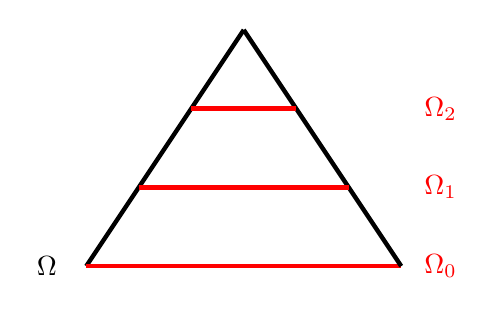
\begin{tikzpicture}
    \draw [ultra thick] (-2,0) -- (0,3);
    \draw [ultra thick, red] (-2,0) -- (2,0);
    \draw [ultra thick] (2,0) -- (0,3);
    \draw [ultra thick, red] (-4/3,1) -- (4/3,1);
    \draw [ultra thick, red] (-2/3,2) -- (2/3,2);
    \draw (2.5,0) [text=red] node {$\Omega_0$};
    \draw (2.5,1) [text=red] node {$\Omega_1$};
    \draw (2.5,2) [text=red] node {$\Omega_2$};
    \draw (-2.5,0) node {$\Omega$};
\end{tikzpicture}
\caption*{Beispiel für ein \((\Omega 1)-(\Omega 2)\)-Gebiet im \(\mathbb{R}^2\)}
\end{subfigure}%
\quad \quad \quad
\begin{subfigure}{.3\textwidth}
\centering
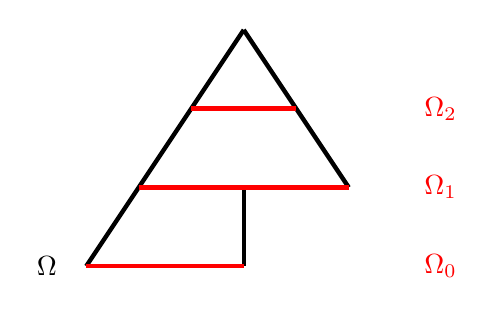
\begin{tikzpicture}
    \draw [ultra thick] (-2,0) -- (0,3);
    \draw [ultra thick] (0,0) -- (0,1);
    \draw [ultra thick, red] (-2,0) -- (0,0);
    \draw [ultra thick] (4/3,1) -- (0,3);
    \draw [ultra thick, red] (-4/3,1) -- (4/3,1);
    \draw [ultra thick, red] (-2/3,2) -- (2/3,2);
    \draw (2.5,0) [text=red] node {$\Omega_0$};
    \draw (2.5,1) [text=red] node {$\Omega_1$};
    \draw (2.5,2) [text=red] node {$\Omega_2$};
    \draw (-2.5,0) node {$\Omega$};
\end{tikzpicture}
\caption*{Beispiel für ein \((\Omega1)\)-Gebiet im \(\mathbb{R}^2\)}
\end{subfigure}
\label{fig:Omega12}
\end{figure}

Wir erinnern uns nun kurz an die Annahmen im \(\Gamma\)-Konvergenzresultat [\ref{theo4.12}, Satz 4.12] zurück. Wir haben dort angenommen, dass \(W\) (H1), (H2), (H4) erfüllt, sowie Norm-koerziv ist ((KO)). Es stellt sich dabei heraus, dass dieser Rahmen die Problemstellung \textbf{stark} vereinfacht. Der Grund ist, dass \(\sigma^*\) durch diese Annahmen einen eindimensionalen Charakter trägt (das liegt insbesondere an (H4)). Wir werden im Folgenden nur die Grundidee skizzieren, da die Details rein technisch (und dabei auch sehr aufwändig) sind und kaum zum intuitiven Verständnis unseres eigentlichen Ziels, dem \(\Gamma\)-Konvergenzresultat [\ref{theo4.12}, Satz 4.12], beitragen. Genau genommen liest sich der Zusammenhang wie folgt:\\[0.5cm]
\pgfsetfillopacity{0.1}\colorbox{generalYellow}{\begin{minipage}{16cm}{\textcolor{black}{\pgfsetfillopacity{1}}{\label{theo4.18}}}
\textbf{Satz 4.18 (\cite{ContiTwoGradientPhase}[Proposition 5.3]):} Unter eben aufgeführten Annahmen an \(W\) gilt:
\begin{equation}
    \sigma^* = \sigma^*_a = \sigma,
\end{equation}
wobei
\begin{equation}
    \sigma = \inf \{ \int_{[-L,L]} W(0,g(s)) + |\frac{dg(s)}{ds}|^2 \,d\lambda^1(s) \, | \, L > 0, \, g \in PC^1([-L,L]), \, g(L) = -g(-L) = a\}.
\end{equation}
\end{minipage}}

\textsc{Beweisidee:}
\begin{enumerate}
    \item Setze \(\{\epsilon_h\} \subset \mathbb{R}^+, \, \{u_h\} \subset W^{2,2}(Q_1,\mathbb{R}^N)\) mit \(\epsilon_h \to 0^+\) fest. (KO) sichert dann die Existenz von:
    \begin{equation}
        \forall t_k \in Q_1 \, \exists C > 0 \, : \, \sup_{k \in \mathbb{N}} |u'(t_k)| \leq C.
    \end{equation}
    Durch die Hölder-Ungleichung und (H1), sowie (H2) erhalten wir dann die gleichmäßige Beschränktheit für zulässige Folgen in \(\sigma^*_a\) in \(W^{1,\infty}(Q_1,\mathbb{R}^N)\). Per Dualität erhalten wir schwache Konvergenz in \(W^{1,1}(Q_1,\mathbb{R}^N)\). 
    \item Indem wir eine p-kompatible Koerzivitätsbedingung in (KO) wählen, erhalten wir dann auch, dass 
    \begin{equation}
    \begin{array}{l}
        \sigma^*_a = \inf \{\liminf_{h \to \infty} \int_{Q_1} \frac{W(0,u'_h)}{\epsilon_h} + \epsilon_h |u^{''}_h|^2 \,d\lambda^1(t) \, | \, \epsilon_h \to 0^+, \, u_h \in W^{2,2}(Q_1, \mathbb{R}^N), \\ 
        u_h \to |t|a \text{ in } W^{1,p}(Q_1, \mathbb{R}^N)\}
    \end{array}
    \end{equation}
    gilt.
    \item Unter der Hinzunahme von (H4), erhält man mit dem Lemma von Fatou und (2) die Behauptung in einem lokalen Fall.
    \item Schließlich ist die eindimensionale Charakterisierung auch für den "globalen" Fall zu zeigen, den man erhält, indem man die lokalen \(\sigma\) aus (3) mittels \(PC^1\)-Kurven \(g\) zu \(\sigma\) "zusammenbaut", i.e. man betrachtet:
    \begin{equation}
        u_h(t) := \int_{[0,t]} v_h (s) \,d\lambda^1(s), \, v_h(t) := \begin{cases}
            -a, \text{ falls }t < -\epsilon_h L \\
            g(\frac{t}{\epsilon_h}), \text{ falls }|t| \leq \epsilon_h L \\
            a, \text{ falls }t > \epsilon_h L
        \end{cases}.
    \end{equation}
    Das ist natürlich genau so konstruiert, dass 
    \begin{equation}
        v_h \to v_0 := \begin{cases}
            -a, \text{ falls }t \leq 0 \\
            a, \text{ falls }t > 0
        \end{cases}
        \text{ in }L^p(Q_1,\mathbb{R}^N) \, \forall p \in [1,\infty[
    \end{equation}
    gilt, also insbesondere:
    \begin{equation}
        u_h \to |t|a \text{ in }W^{1,p}(Q_1,\mathbb{R}^N).
    \end{equation}
\end{enumerate}
Für die Details verweisen wir auf \cite{ContiTwoGradientPhase} [Proposition 5.1, Corollary 5.2, Proposition 5.3]. \QEDB

Nun befinden wir uns in der Situation, das \(\Gamma\)-Limsupresultat für den \((\Omega1)-(\Omega2)\)-Fall zu beweisen:\\[0.5cm]
\pgfsetfillopacity{0.1}\colorbox{generalYellow}{\begin{minipage}{16cm}{\textcolor{black}{\pgfsetfillopacity{1}}{\label{theo4.19}}}
\textbf{Satz 4.19 (\cite{ContiTwoGradientPhase}[Theorem 5.5]):} Angenommen, \(\Omega\) erfüllt \((\Omega1)\) und \((\Omega2)\), \(W\) (H1), (H2), (KO) und (H4). Sei \(u \in W^{1,1}(\Omega,\mathbb{R}^N)\) mit \(Du \in \mathcal{BV}(\Omega,\{A,B\})\). Dann gilt für \(\{\epsilon_h\} \subset \mathbb{R}^+\) mit \(\epsilon_h \to 0^+\), \(E \subset \mathcal{M}^n(\mathbb{R}^n)\):
\begin{equation}
    \Gamma-\limsup_{h \to \infty} \mathcal{I}_{\epsilon_h} (u,\Omega) \leq \sigma^* |D \chi_E| (\Omega),
\end{equation}
wobei \(Du = (1 - \chi_E(x))A + \chi_E (x) B\) \(\lambda^n\)-f.ü.
\end{minipage}}

\textsc{Beweis:} Annahme \((\Omega1)\) validiert die Anwendung von \eqref{eq4.81}, i.e. es gilt:
\begin{equation}
    u(x) = \tilde{u}(x_n) = f_0 + a x_n - 2h(x_n)a \, \lambda^n-\text{f.ü.}
\end{equation}
mit \(h \in W^{1,\infty}(\mathbb{R}), \, h' \in \mathcal{BV}(\mathbb{R},\{0,1\})\),
\begin{equation}
    S(Du) \cap \Omega = \bigcup_{i=1}^{\infty} \Omega_{l_i},
\end{equation}
wobei \(\Omega_{l_i} := \{(x',x_n) \in \Omega \, | \, x_n = l_i\}\), \(l_i \in \mathbb{R}\).\\
\textbf{Schritt 1:} Angenommen, \(S(Du) \cap \Omega = \bigcup_{i=1}^k \Omega_{l_i}, \, k \in \mathbb{N}\) beliebig, aber fest, sowie o.B.d.A. seien \(l_i\) aufsteigend total geordnet, i.e. \(l_1 < ... < l_k\). Um die Behauptung zu beweisen, wissen wir nach [\ref{theo4.18}, Satz 4.18], dass es reicht, die Behauptung für \(\sigma\), statt \(\sigma^*\) zu zeigen. Wir wählen also jetzt in diesem Rahmen Kurven \(g_j \in PC^1([-L,L],\mathbb{R}^N)\) mit \(g_j(L) = -g_j(L) = a\), sodass
    \begin{equation}{\label{eq4.120}}
        \int_{[-L,L]} W(0,g_j(s)) + |g^{\prime}_k(s)|^2 \,d\lambda^1(s) \leq \sigma + \frac{1}{j}
    \end{equation}
    gilt. O.B.d.A. wähle \(\epsilon_h\) so klein, dass \(l_i + \epsilon_h L < l_{i+1} - \epsilon_h L\) (durch ein typisches Skalierungsargument kann man diesen Rahmen immer erzwingen) für \(i=1,...,k-1\). Definiere:
    \begin{equation}{\label{eq4.121}}
        v_{\epsilon_h,j}(s) := \begin{cases}
            g_j(-sgn(u^{\prime}(l_i - \epsilon_h L) \cdot a) \frac{s-l_i}{\epsilon_h}), \text{ falls } s \in ]l_i - \epsilon_h L, l_i + \epsilon_h L[, \, i=1,...,k \\
            \tilde{u}^{\prime}(s), \text{ sonst in }\mathbb{R}
        \end{cases},
    \end{equation}
    wobei wir \(\tilde{u}^{\prime}\) stetig auf ganz \(\mathbb{R}\) fortgesetzt haben (der dafür nötige stetige Fortsetzungsoperator existiert dank des \(C^1\)-Randes des Intervalls \(]l_1- \epsilon_h L, \, l_k + \epsilon_h L[\), vergleiche hier das klassische Sobolevresultat). Dem zugrundeliegend setzen wir dann:
    \begin{equation}
        u_{\epsilon_h,j}(x) = \tilde{u}_{\epsilon_h,j} (x_n) := \tilde{u}(l_1) + \int_{[x_n,l_1]} v_{\epsilon_h,j}(s) \,d\lambda^1(s).
    \end{equation}
    Dann gilt:
    \begin{equation}
    \begin{array}{l}
        \int_{\Omega} |Du_{\epsilon_h,j} - Du| \,d\lambda^1(x) \stackrel{(\ref{eq4.121})}{\leq} C \sum_{i=1}^k \int_{[l_i - \epsilon_h L, l_i + \epsilon_h L]}|g_j(\pm \frac{s-l_i}{\epsilon_h})| + 1 \,d\lambda^1(s) \stackrel{(*)}{\leq} \\
        2Cm \epsilon_h L + C \sum_{i=1}^k \epsilon_h \int_{[-L,L]} |g_j (t)| \,d\lambda^1(t),
    \end{array}
    \end{equation}
    wobei (*) valide ist, da gilt:
    \begin{equation}
        \lim_{s \to (l_i \pm \epsilon_h L)} |g_j(\pm \frac{s-l_i}{\epsilon_h}| \stackrel{Stet.}{=} a < 2a = |g_j(L) - g_j(-L)| \stackrel{C-S}{\leq} \int_{[-L,L]} |g^{\prime}_j(s)| \,d\lambda^1(s).
    \end{equation}
    Mit der Poincare-Ungleichung erhalten wir dann, dass
    \begin{equation}{\label{eq4.125}}
        u_{\epsilon_h,j} \stackrel{\epsilon_h \to 0^+}{\to} u \text{ in }W^{1,1}(\Omega,\mathbb{R}^N)
    \end{equation}
    gilt. Zusammengefasst erhalten wir:
    \begin{equation}
    \begin{array}{l}
        \lim_{\epsilon_h \to 0^+} \mathcal{I}_{\epsilon_h} (u_{\epsilon_h,j},\Omega) \stackrel{Def.}{=} \\
        \lim_{\epsilon_h \to 0^+} \sum_{i=1}^k \int_{\Omega \cap \{l_i + \epsilon_h L < x_n < l_{i+1} + \epsilon_h L\}} \frac{W(0,g_j(\pm \frac{x_n - l_i}{\epsilon_h}))}{\epsilon_h} + \frac{1}{\epsilon_h} |g^{\prime}_j (\pm \frac{x_n - l_i}{\epsilon_h})|^2 \,d\lambda^1(x) \stackrel{Cav.}{=} \\
        \lim_{\epsilon_h \to 0^+} \sum_{i=1}^k \int_{[l_i - \epsilon_h L, l_i + \epsilon_h L]} (\frac{W(0,g_j(\pm \frac{s - l_i}{\epsilon_h}))}{\epsilon_h} + \frac{1}{\epsilon_h} |g^{\prime}_j (\pm \frac{s - l_i}{\epsilon_h})|^2) \mathcal{H}^{n-1}(\{x \in \Omega \, | \, x_n = s\}) \,d\lambda^1(s) \stackrel{(\ref{eq4.125})}{=}\\
        \lim_{\epsilon_h \to 0^+} \sum_{i=1}^k \int_{[-L,L]} (W(0,g_j(t)) + |g^{\prime}_j(t)|^2) \mathcal{H}^{n-1}(\{x \in \Omega \, | \, x_n = \epsilon_h t + l_i \})\,d\lambda^1(t) \stackrel{(\Omega2)}{=} \\
        (\int_{[-L,L]} W(0,g_j(t)) + |g^{\prime}_j (t)|^2 \,d\lambda^1(t)) \sum_{i=1}^k \mathcal{H}^{n-1}(\Omega_{l_i}) \stackrel{(\ref{eq4.120})}{\leq} (\sigma + \frac{1}{j}) \sum_{i=1}^k \mathcal{H}^{n-1}(\Omega_{l_i}).
    \end{array}
    \end{equation}
    Betrachten wir dann \(\limsup_{j \to \infty}\), so erhalten wir die Behauptung.\\
\textbf{Schritt 2:} Angenommen, \(S(Du) \cap \Omega = \bigcup_{i=1}^{\infty} \Omega_{l_i}\). Dann erhalten wir die Behauptung limitisch aus Schritt 1, da für einen Häufungspunkt \(l\) von \(\{l_i\}\) gilt, dass \(l \in \{\alpha,\beta\}\).\\[0.2cm]
    \textit{Begründung, dass das gilt: Angenommen, das wäre falsch, so gilt für \(\Omega_l \neq \emptyset\), dass ein \(x = (x',l) \in \Omega\) existiert und \(B_{r}(x') \, \times ]l-d,l+d[ \subset \Omega\) offen (bezüglich der euklidischen Relativtopologie) für \(d \in \mathbb{N}\). Für \(i_j\) groß genug, ist auch \(B_{r}(x') \, \times \{l_{i_j}\} \subset \Omega\) offen (bezüglich der euklidischen Relativtopologie), wobei \(\{l_{i_j}\} \to l\) und damit:
    \begin{equation}
        \infty > \sum_{i=1}^{\infty} \mathcal{H}^{n-1} (\Omega_{l_i}) \geq \sum_{i_j} \mathcal{H}^{n-1}(B_{r}(x')) = \infty.
    \end{equation}
    }\\[0.2cm]
    Sei also nun wieder \(k \in \mathbb{N}\) beliebig, aber fest. Definiere:
    \begin{equation}
        U_k := \{x \in \Omega \, | \, \alpha + \delta_k < x_n < \beta - \delta_k\},
    \end{equation}
    wobei \(\delta_k \to 0^+\), also \(\{l_i\} \cap \{\alpha + \delta_k, \beta - \delta_k\} \stackrel{s.o.}{=} \emptyset\). Damit gilt \(\lambda^n(\Omega \textbackslash U_k) \stackrel{k \to \infty}{\to} 0\) und die Behauptung folgt aus Schritt 1. 
Damit ist die Behauptung gezeigt. \QEDB
%%%%%%%%%%%%%%%%%%%%%%%%%%%%%%%%%%%%%%%%%%%%%%%%%%%%%%%%%%%%%%%%%%%%%%%%%%%%
\subsection[Verbesserungen des Conti-Fonseca-Leoni Modells: Der Weg zur SO(N)-Invarianz]{Verbesserungen des Conti-Fonseca-Leoni Modells: Der Weg zur SO(\(\mathbb{N}\))-Invarianz}{\label{subsec:soninva}}
Wir erinnern nun noch einmal an die Annahmen, die im letzten Unterkapitel getroffen wurden (Definitionen wie gehabt):
\begin{itemize}
    \item (H1) \(\exists a \in \mathbb{R}^N \, \textbackslash \{0\} \, : \, A -                 B = a \otimes \nu\),
    \item (H2) W ist stetig, \(\{W = 0\} = \{A,B\}\),
    \item (H3) \(\exists C > 0 \, \forall z \in \mathbb{R}^{N \times n} \, : \,                 W(z) \geq C |z| - \frac{1}{C}\).
    \item (H4) \(W(z) \geq W(0,z_n)\) mit \(z = (z',z_n) \in \mathbb{R}^{N                      \times (n-1)} \times \mathbb{R}^N\).
\end{itemize}
Wir hatten in [\ref{prop4.11}, Proposition 4.11] begründet, dass (H1) im Allgemeinen keine große Einschränkung darstellt. Auch (H3) ist keine zu große Einschränkung, denn ohne jegliche Wachstumsschranken ist generell keine \(\Gamma\)-Konvergenz zu erwarten. Allerdings sind der zweite Teil von (H2) ((H2)-2) und (H4) sehr störend. (H2)-2 erzeugt ein starres Modell, da jegliche Oszillationen zwischen den einzelnen Potentialen komplett vernachlässigt wird. (H4) ist hierbei aber die stärkste Einschränkung, da sie eine Kontrolle durch ein eindimensionales Problem annimmt. Wir werden nun aktuelle Forschungsergebnisse aufführen, die sich mit diesen Problemen befasst haben. Dabei werden wir aber nur die neuen Ideen aufführen, Details lassen sich dann in den \\jeweiligen Quellen finden.

\subsubsection{Schritt 1: SO(2)-Invarianz nach S. Conti und B. Schweizer in \cite{conti2006rigidity}}
Wir modifizieren die Bedingungen nun also zu:
\begin{itemize}
    \item (H1)' \(\exists a \in \mathbb{R}^2 \, : \, A-QB = a \otimes \nu\),
    \item (H2)' \(W \in C(\mathbb{R}^{2 \times 2}) \, : \, (W(QF) = W(F) \, \forall F \in \mathbb{R}^{2 \times 2}, \, Q \in SO(2) \, \land \, \{W = 0\} = K := SO(2)A \cup SO(2)B)\),
    \item (H3)' \(c_1 d_{Fr}^2(F,K) \leq W(F) \leq c_2 d_{Fr}^2(F,K)\) (Fr steht hier für Frobenius; die Metrik ist also die von der Frobenius-Norm induzierte.),
\end{itemize}
wobei \(det \, A > 0, \, det \, B > 0, \, c_1, \, c_2 > 0\). S. Conti und B. Schweizer bewiesen auf dieser Grundlage folgendes Theorem:\\[0.5cm]
\pgfsetfillopacity{0.1}\colorbox{generalYellow}{\begin{minipage}{16cm}{\textcolor{black}{\pgfsetfillopacity{1}}{\label{theo4.20}}}
\textbf{Satz 4.20 (\cite{conti2006rigidity}[Theorem 3.1]):} Angenommen, \(\Omega \subset \mathbb{R}^2\) ist ein strikt sternförmiges, beschränktes Lipschitz-Gebiet, in dem (H1)', (H2)' und (H3)' erfüllt sind. Dann gilt für \(u \in W^{1,1}(\Omega, \mathbb{R}^2)\):
\begin{equation}
    \Gamma-\lim_{\epsilon \to 0} \mathcal{I}_{\epsilon} (u,\Omega) = \mathcal{I}_0(u,\Omega) := \begin{cases}
        \sigma^* \mathcal{H}^1(S(Du) \cap \Omega), \text{ falls } Du \in \mathcal{BV}(\Omega,K) \\
        \infty, \text{ sonst}
    \end{cases},
\end{equation}
wobei
\begin{equation}
    \sigma^* := \inf \{\liminf_{h \to \infty} \mathcal{I}_{\epsilon_h} (u_h,Q_{\nu}) \, | \, \epsilon_h \to 0, \, u_h \to u_0 \text{ in }L^1(Q_2,\mathbb{R}^N)\}
\end{equation}
und
\begin{equation}
    Du_0 := \begin{cases}
        A, \text{ falls } x \cdot \nu > 0 \\
        QB, \text{ falls } x \cdot \nu < 0
    \end{cases}.
\end{equation}
\end{minipage}}

\textsc{Beweisidee:} Wie üblich benötigen wir wieder ein Kompaktheits- \(\Gamma\)-liminf und \(\Gamma\)-limsup Resultat:
\begin{itemize}
    \item \textbf{Kompaktheit:} Wir halten zunächst fest (das Ursprungsresultat ist in \cite{ball1984w1} zu finden): Ist eine Lebesgue-integrable Funktion \(g : \mathbb{R} \to \mathbb{R}\) periodisch auf einem Ball \(B_r(x)\) durch eine lokal Lebesgue-integrable Funktion \(h:\mathbb{R}^n \to \mathbb{R}\) fortgesetzt, so gilt für eine Borelmenge \(E\), sowie
    \begin{equation}
        w_j := h(jx),
    \end{equation}
    dass \(w_j\) ein Young-Maß \(\vartheta_x \in \mathcal{Y}(\Omega,\mathbb{R}^N)\) erzeugt, für das gilt:
    \begin{itemize}
        \item \(\int_{\mathbb{R}} g \,d\vartheta_x = \int_{B_r(x)} g(h(y)) \,d\lambda^n(y)\),
        \item \(\vartheta_x(E) = \lambda^n(B_r(x) \cap h^{-1}(E))\).
    \end{itemize}
    Damit ist klar, dass gilt:
    \begin{equation}
        \int_{B_r(x)} \vartheta_x(SO(n)B) \,d\lambda^n(x) = \lambda^n(B_r(x) \cap E).
    \end{equation}
    Der Träger von dem für unseren Rahmen erzeugte Young-Maß \(\vartheta_x\) ist wieder in einer kompakten Menge, weshalb wir das Kompaktheitsresultat schließen können, wenn wir zeigen, dass für Lebesgue-Punkte \(x_0\) der Dichte 0 zeigen, dass \(Du_0(x_0) \in SO(n)A\) gilt (da wir nach [\ref{lem2.3}, Lemma 2.3] wissen, dass für \(L^1\)-Funktionen \(\lambda^n\)-f.a. Punkte der Funktion Lebesgue-Punkte sind). Kurz gesagt ist das korrekt, da die Hilfsfunktion
    \begin{equation}
        \phi(z) := ||z||^n_{Fr} - n^{n/2} det \,z
    \end{equation}
    polykonvex ist (valide, da für \((2 \times 2)\)-Matrizen die Determinante polykonvex ist (aber \textbf{nicht} konvex!)).
    \item \textbf{\(\Gamma\)-Liminf:} Da wir für die Wachstumsbeschränkung nach unten den nahezu identischen Rahmen vorliegen haben, ist der Beweis fast identisch zu dem von [\ref{theo4.15}, Satz 4.15]. Die Idee ist es, Rechtecke zwischen den "Schnittstellen" (also an dem Übergang von Phase A zu Phase B bzw. vice versa) auf \(S(Du)\) zu betrachten und schlussendlich die Unabhängigkeit der Größe der Rechtecke zu zeigen.
    \item \textbf{\(\Gamma\)-Limsup:} Wie immer ist dieser Schritt der mit Abstand schwierigste. Die Idee ist hier, um
    \begin{equation}
        \mathcal{I}_{\epsilon_h}(u_h,\Omega) \to \mathcal{I}_0(u_0,\Omega)
    \end{equation}
    für \(u_h \to u_0\) zu erhalten, limitische Funkten zu betrachten, die endlich viele Schnittstellen besitzen, die nicht auf dem Rand liegen (diese Approximation ist valide, da sie dicht in \(\Omega\) liegt). \QEDB
\end{itemize}

\subsubsection{Schritt 2: SO(\(\mathbb{N}\))-Invarianz nach E. Davoli und M. Friedrich in \cite{davoli2020two}}
Als nächsten Schritt bewiesen E. Davoli und M. Friedrich den allgemeinen Fall, jedoch unter Hinzunahme eines anisotropischen Regularitätstermes, i.e. das Energiefunktional
\begin{equation}
    \mathcal{E}_{\epsilon,\eta} := \begin{cases}
        \mathcal{I}_{\epsilon} (u,\Omega) + \eta^2 \int_{\Omega} ||D^2 u||_{Fr}^2 - |\partial_n^2 u|^2 \,d\lambda^n(x), \text{ falls }u \in W^{2,2}(\Omega,\mathbb{R}^n) \\
        \infty, \text{sonst}
    \end{cases},
\end{equation}
wobei \(\eta > 0\). Als zweite Einschränkung modifizieren wir jetzt noch (H1) zu:
\begin{itemize}
    \item (H1) \(\exists a \in \mathbb{R}^n \textbackslash \{0\} : B - A = a e_n \otimes e_n\).
\end{itemize}
Wir haben bereits in [\ref{prop4.11}, Proposition 4.11] gesehen, dass (H1) keine allzugroße Einschränkung darstellt, so auch hier. Wir führen nun die wesentlichen neuen Ideen auf zu dem Conti-Resultat [\ref{theo4.13}, Satz 4.13]. Diese beschränken sich rein auf den Beweis des \(\Gamma\)-Limsup. Im Folgenden nehmen wir stets für die Phasenseperation die Wachstumsschranke:
\begin{equation}
    \int_{\Omega} W(Du) \,d\lambda^n(x) \leq C \epsilon^2, \, C > 0
\end{equation}
an. Bisherige Resultate befassten sich mit einem komplett starren Modell ([\ref{theo4.12}, Satz 4.12]) oder nahmen nur Rücksicht auf \textbf{eines} der beiden Potentiale. Letzteres umfasst z.B. Modelle mit stark inkompatiblen Potentialen (\cite{de2006simple}, \cite{chaudhuri2004rigidity}; für diese Arbeit irrelevant, da hier offensichtlich \textbf{keine} Phasentrennung entsteht (das sieht man sogar mathematisch: für \(\epsilon \ll 1\) ist \(Du \sim F \in \mathbb{R}^{n \times n}\))). Um beide (kompatiblen) Potentiale simultan modellieren zu können, benötigen wir eine Art "Indikator", um dynamisch die "aktive" Phase jeweils zu betrachten. Genau solch einen "Phasen-Indikator" führten E. Davoli und M. Friedrich in \cite{davoli2020two} ein: Wir werden diesen im Folgenden mit \(\mathcal{M} \in \mathcal{BV}(\Omega, \{A,B\})\) bezeichnen. Damit wir das Conti-\(\Gamma\)-Konvergenz Resultat [\ref{theo4.20}, Satz 4.20] in allgemeiner Dimension erreichen können, müssen wir einen passenden Rahmen finden, der uns die korrekten sogenannten "Starrheits Abschätzungen" (Englisch: rigidity estimates) liefert. Korrekt heißt in dem Zusammenhang eine Abschätzung der Form:
\begin{equation}{\label{eq4.138}}
    \exists R \in SO(n) \, : \, ||Du - R\mathcal{M}||_{L^2(\Omega)} \leq C \epsilon.
\end{equation}

\textbf{Bemerkung:} Die Ordnung \(\epsilon\) ist wichtig, da Verzerrung in fest-fest Phasenübergängen in den allermeisten Fällen von genau dieser Ordnung auftritt! Beispielsweise haben R. Jerrard und A. Lorent in \cite{jerrard2013multiwell} unter der Annahme von:
\begin{equation}{\label{eq4.139}}
    ||D^2 u||_{L^1(\Omega)} \leq C_1, \, 0 < C_1 < 1,
\end{equation}
gezeigt, dass die Folgende Abschätzung gilt:
\begin{equation}
    ||Du - R\{A,B\}||_{L^2(\tilde{\Omega})} \leq C \sqrt{\epsilon},
\end{equation}
wobei \(\tilde{\Omega} \subset \Omega\). Das Resultat kann im Allgemeinen \textbf{nicht} auf ganz \(\Omega\) erweitert werden; Grund hierfür sind hier nicht ausgeschlossene, mögliche Phasenübergänge nahe des Randes von \(\Omega\). \(C_1\) ist hier derart klein in \eqref{eq4.139} gefordert, um die Dominanz der \(\{A,B\}\)-Phasenregion zu garantieren. Die Ordnung der Abschätzung passt aber nicht und noch schlimmer: es kann sogar gezeigt werden, dass diese Schranke scharf ist, siehe \cite{davoli2020two}[Remark 3.9].

Wir geben hier nun das entscheidende Starrheits Resultat an, das gleichzeitig auch zeigt, warum der zusätzliche \(\eta\)-Stabilitätsterm in \(\mathcal{E}_{\epsilon, \eta}\) unter ähnlichen Annahmen wie im Conti-Fall, i.e. wir nehmen an, dass gilt:
\begin{itemize}
    \item (H1)' : Siehe oben;
    \item (H2) : \(W : \mathbb{R}^{n \times n} \to [0,\infty[\) ist stetig;
    \item (H3) : \(W(RF) = W(F)\) für alle \(R \in SO(n), \, F \in \mathbb{R}^{n \times n}\);
    \item (H4) : \(W(\mathbb{1}) = W(diag(1,...,1,1 + \kappa))\) für \(\kappa > 0\);
    \item (H5) : \(\exists C_2 > 0 \, \forall F \in \mathbb{R}^{n \times n} \, : W(F) \geq C_2 d_{Fr}^2(F,SO(n)\{A,B\})\),
\end{itemize}
nötig ist:\\[0.5cm]
\pgfsetfillopacity{0.1}\colorbox{generalYellow}{\begin{minipage}{16cm}{\textcolor{black}{\pgfsetfillopacity{1}}{\label{theo4.21}}}
\textbf{Satz 4.21 (\cite{davoli2020two}[Theorem 3.1]):} Angenommen, (H1)', sowie (H2) - (H5) gelten. Wir unterscheiden:
\begin{enumerate}
    \item \textbf{(Dimension 2):} Sei \(\Omega\) ein beschränktes, einfach zusammenhängendes Lipschitz Gebiet in \(\mathbb{R}^2\), \(\eta \geq \epsilon > 0\). Dann existiert eine Konstante \(C = C(\Omega,\kappa,C_2)\) > 0, sodass für alle \(u \in W^{2,2}(\Omega,\mathbb{R}^2)\) ein \(R \in SO(2)\) existiert mit:
    \begin{equation}
        ||Du - R \mathcal{M}||_{L^2(\Omega)} \leq C \epsilon \sqrt{\mathcal{E}_{\epsilon,\eta}(u)} + C (\frac{\epsilon}{\eta} + \frac{\epsilon^{1/2}}{\eta^{3/2}}) \mathcal{E}_{\epsilon,\eta}(u).
    \end{equation}
    \item \textbf{(Dimension \(\geq 3\)):} Sei \(\Omega\) ein beschränktes Lipschitz Gebiet in \(\mathbb{R}^n\) mit \(n \geq 3\). Sei zudem \(p \in [1,2]\), \(p \neq \frac{n}{n-1}\), \(\eta \geq \epsilon > 0\). Dann existiert für alle \(\tilde{\Omega} \in \overline{K}(\Omega)\) eine Konstante \(C = C(\Omega, \tilde{\Omega}, \kappa, p, C_2) > 0\), sodass für alle \(u \in W^{2,2}(\Omega,\mathbb{R}^n)\) ein \(R \in SO(n)\) existiert mit:
    \begin{equation}
        ||Du - R \mathcal{M}||_{L^p(\tilde{\Omega})} \leq C \epsilon \sqrt{\mathcal{E}_{\epsilon,\eta}(u)} + C ((\frac{\epsilon}{\eta} + \frac{\epsilon^{1/2}}{\eta^{3/2}}) \mathcal{E}_{\epsilon,\eta}(u))^{\theta},
    \end{equation}
    wobei \(\theta := \min \{1,\frac{n}{p(n-1)}\}\).
\end{enumerate}
In beiden Fällen gilt zudem:
\begin{equation}
    |D\mathcal{M}|(\Omega) \leq C \mathcal{E}_{\epsilon,\eta}(u).
\end{equation}
\end{minipage}}

\textbf{Bemerkung:} Auch in (2) kann das Resultat im Allgemeinen wieder nicht auf ganz \(\Omega\) erweitert werden. Der Beweis nutzt diesen Aspekt in dem Sinne aus, dass er per Approximation die Aussage auf einer Überdeckung mit (bezüglich der euklidischen Relativtopologie) offenen Quadern zeigt (diese endliche Teilüberdeckung ist möglich, da \(\mathbb{R}^n\) total beschränkt ist und in \(\mathbb{R}^n\) alle Normen äquivalent sind). Generell sieht man an dem Resultat schon auftretende Probleme in höheren Dimensionen als 2; wir werden später in \ref{sec:gendim} noch genauer darauf eingehen, warum das Verallgemeinern der Conti-Beweis-Strategie in [\ref{theo4.20}, Satz 4.20] alles andere als einfach ist.
%%%%%%%%%%%%%%%%%%%%%%%%%%%%%%%%%%%%%%%%%%%%%%%%%%%%%%%%%%%%%%%%%%%%%%%%%%%%%%%%%%%%%%%%%%%%%%%%%%%%%%%%%%%%%%%%%%%%%%%%%%%%%%%%%%%%%%%%%%%%
\section{Physikalischer Exkurs: Doppelter Potentialtopf}{\label{sec:exwell}}
Dieser Exkurs beschäftigt sich mit der Physik hinter dem doppelten Potentialtopf. Quantenmechanische Grundlagen werden hierfür vorausgesetzt; für das Verständnis der Arbeit ist dieser Exkurs allerdings rein optional.\\

Wir erinnern uns an den unendlichen Potentialtopf aus der Quantenmechanik und modifizieren diesen nun. Diesem ist geschuldet, dass wir zwei nicht homogene Stoffe vorliegen haben, weshalb wir im Modell quantenmechanisch zwei "aneinanderhängende" Potentialtöpfe mit Tunneling Effekten betrachten müssen, i.e. Teilchen tunneln durch die Barriere der beiden Potentiale. Physikalisch ist der Übergang zwischen den beiden Stoffen deshalb nicht-trivial und die Eigenenergien der Potentialtöpfe werden durch Tunneling Effekte bedeutend beeinflusst. Als Beispiel werden wir nun das Problem aus \cite{DoubleWellBerdecia} betrachten:\\
Wir betrachten ein Teilchen der Masse m mit Potential
\begin{equation}
    V : \mathbb{R} \to \mathbb{R}, \, V(x) := \alpha x^4 - \beta x^2 + \gamma \, \, \forall \alpha > 0 \, \forall \beta > 0,
\end{equation}
wobei \(\gamma = \frac{\beta^2}{4 \alpha}\) die Höhe der Potentialbarriere darstellt. In diesem Rahmen lässt sich die Schrödinger-Gleichung schreiben als
\begin{equation}
    (\mathbb{H} - \eta) \Psi(x) = 0,
\end{equation}
wobei der Hamilton Operator \(\mathbb{H}\) und \(\eta\) hier definiert sind als:
\begin{equation}
    \mathbb{H}x := \frac{d^2}{dx^2} - (\frac{2m}{\hbar^2})V(x), \, \eta := -(\frac{2mE}{\hbar^2})
\end{equation}
mit der Energie E. Graphisch entspricht dieser Rahmen folgender Vorstellung:
\begin{figure}[label={fig:dwp}, caption={Ein Beispiel für einen eindimensionalen Doppelpotentialtopf in symmetrischer Form \cite{DoubleWellBerdecia}}]
    \includegraphics[scale=0.5]{figures/DoubleWellPot.pdf}
\end{figure}

Unser Ziel ist es im nächsten Kapitel, als Anwendung ein variationelles Modell für Lithium-Ionen Akkus (genauer: LiFePO\(_4\) (Lithium-Eisenphosphat) Akkumulatoren) zu betrachten. Bevor wir diesbezüglich das variationelle Modell mathematisch unter die Lupe nehmen, stellt sich aus diesem Exkurs zunächst einmal die Frage heraus: Wie überträgt sich hier die Rolle des doppelten Potentialtopf physikalisch? H. Federmann, M. Fleck und H. Emmerich von der Universität Bayreuth haben sich genau diese Frage gestellt und ihre Ergebnisse in \cite{LiFedermann} festgehalten:\\
Der hier benutzte Ansatz wird als Phasenfeldmethode bezeichnet. Sie ist die physikalische Beschreibung der mathematischen Theorie der Phasenübergänge. In einem Lithium-Ionen Akku findet ein Phasenübergang an der Elektrode statt: Je nachdem, ob Lithium deinsertiert oder insertiert wird, entstehen verschiedene Phasen. Den Prozess der Desinsertion und Insertion kann man sich folgendermaßen vorstellen:
\newpage
\begin{figure}[label={fig:lidesint}, caption={Der Prozess der Lithium Desinsertion/Insertion graphisch dargestellt \cite{LiFedermann}}]
    \includegraphics[scale=0.5]{figures/LithiumAkkus.pdf}
\end{figure}

Die Verbindung bezüglich des doppelten Potentialtopfs ist dann wie folgt:\\
Sei \(\Phi : \mathbb{R}^n \times \mathbb{R} \to \{0,1\}, \, (x,t) \mapsto \Phi(x,t)\) das Phasenfeld, welches den Wert 0 für Lithium arme Phasen und 1 für Lithium reiche Phasen annimmt. Die Grenzflächenenergie wird dann beschrieben durch:
\begin{equation}
    \mathcal{E}_g (\Phi) = \frac{3 \mathcal{E}_o b}{2} (\nabla \Phi)^2 + \frac{6 \mathcal{E}_o}{b} W(\Phi),
\end{equation}
wobei \(W(\Phi) = \Phi^2(1-\Phi)^2\) dem zugehörigen doppelten Potentialtopf entspricht und \(\mathcal{E}_o\) die Oberflächenenergie, sowie b die Breite der Grenzfläche darstellen.